%%%%%%%%%%%%%%%%%%%%%%%%%%% asme2ej.tex %%%%%%%%%%%%%%%%%%%%%%%%%%%%%%%
% Template for producing ASME-format journal articles using LaTeX    %
% Written by   Harry H. Cheng, Professor and Director                %
%              Integration Engineering Laboratory                    %
%              Department of Mechanical and Aeronautical Engineering %
%              University of California                              %
%              Davis, CA 95616                                       %
%              Tel: (530) 752-5020 (office)                          %
%                   (530) 752-1028 (lab)                             %
%              Fax: (530) 752-4158                                   %
%              Email: hhcheng@ucdavis.edu                            %
%              WWW:   http://iel.ucdavis.edu/people/cheng.html       %
%              May 7, 1994                                           %
% Modified: February 16, 2001 by Harry H. Cheng                      %
% Modified: January  01, 2003 by Geoffrey R. Shiflett                %
% Use at your own risk, send complaints to /dev/null                 %
%%%%%%%%%%%%%%%%%%%%%%%%%%%%%%%%%%%%%%%%%%%%%%%%%%%%%%%%%%%%%%%%%%%%%%

%%% use twocolumn and 10pt options with the asme2ej format
\documentclass[twocolumn,10pt]{asme2ej}

\usepackage{epsfig} %% for loading postscript figures
\usepackage{amsmath}

\graphicspath{{./}{./FIGURES/}}
\usepackage{listings}
\usepackage[colorlinks, linkcolor=blue, citecolor=blue, filecolor=black,urlcolor=blue]{hyperref}


\newcommand{\be}[1]{ \begin{equation} \label{#1}}
\newcommand{\ee}{\end{equation}}


\newcommand{\bes}[1]{ \begin{equation} \label{#1}\begin{array}{rl}}
\newcommand{\ees}{\end{array}\end{equation}}



%% The class has several options
%  onecolumn/twocolumn - format for one or two columns per page
%  10pt/11pt/12pt - use 10, 11, or 12 point font
%  oneside/twoside - format for oneside/twosided printing
%  final/draft - format for final/draft copy
%  cleanfoot - take out copyright info in footer leave page number
%  cleanhead - take out the conference banner on the title page
%  titlepage/notitlepage - put in titlepage or leave out titlepage
%  
%% The default is oneside, onecolumn, 10pt, final


%\title{Popularizing linear and nonlinear global approaches to hydrodynamic instabilities : 
%A review and a simple implementation for the wake of a cylinder}

\title{A {practical} review on linear and nonlinear global approaches to stability analysis}

%%% first author
\author{D. Fabre$^{(a)}$, D. Ferreira Sabino$^{(a)}$, P. Bonnefis$^{(a)}$,  V. Citro \& F. Giannetti
    \affiliation{
	IMFT, University of Toulouse
    }	
}

%%% second author
%%% remove the following entry for single author papers
%%% add more entries for additional authors
%\author{V. Citro$^{(b)}$ \& F. Giannetti$^{(b)}$ \\
 %   \affiliation{ University of Salerno
  %  }
%}

\usepackage{cprotect}

\begin{document}
\lstset{numbers=left, numberstyle=\small, numbersep=8pt, frame = single, language=Matlab, framexleftmargin=15pt}

\maketitle    

%%%%%%%%%%%%%%%%%%%%%%%%%%%%%%%%%%%%%%%%%%%%%%%%%%%%%%%%%%%%%%%%%%%%%%
\begin{abstract}
{\it 
This paper is aimed to review the linear and nonlinear approaches to study the stability of fluid flows. 
We provide a concise but self-contained exposition of the main concepts and specific numerical methods 
designed for global stability studies, including the classical linear stability analysis, the adjoint-based sensitivity and  
the most recent nonlinear developments.
A simple computer code, that implements all the concepts discussed in the present paper, is provided. 
In particular, we discuss the mesh adaptation, the use of simple shift-invert strategy instead of the classical Arnoldi algorithm and a reformulation and simplification of the recent nonlinear self-consistent approach proposed by Manti\v{c}-Lugo et al \cite{MLugo2014} in terms of a harmonic balance. The code is demonstrated for the reference case of the incompressible, two-dimensional flow around a circular cylinder, but the software is easily customisable to a variety of other 
flow configurations or flow equations.
%An abstract for an ASME paper should be less than 150 words and is normally in italics.
}
\end{abstract}

%%%%%%%%%%%%%%%%%%%%%%%%%%%%%%%%%%%%%%%%%%%%%%%%%%%%%%%%%%%%%%%%%%%%%%


\section{Introduction}

The concept of stability bears on the reaction of a system to a small perturbation of its state. If the generic disturbance grows in time, the system is unstable. The concept of stability can be simply formulated for a system of Ordinary Differential Equations (ODE). 
Such systems can be at equilibrium, where the state does not depend on time, or can present a periodic state, with all components returning to the same values, after every period. 

The stability of fluid flows usually depends on the value of a given parameter. A bifurcation occurs when a critical value is reached and the original solution becomes linearly unstable, with the system tending towards a new steady or unsteady state. 
%The destabilization of a flow as a parameter is varied, leading from a steady solution to a unsteady one, is an ubiquous situation in fluid dynamics. 
In the second part of the 19th century, specific analytical and numerical methods able to study these bifurcations have emerged and are continuously evolving up to the present days. 
A crucial point, that drove the development in this field, is the availability of larger and larger computing resources. 
Initially, the linear stability theory focused on fluid flows that are homogeneous in two spatial directions, e.g. plane Poiseuille flow \cite{Dreid2004}. This implies that the streamwise and the spanwise base-flow gradients vanish and, as a consequence, it is possible to consider only one (streamwise) velocity component. Thus, the stability problem requires a \textit{local} numerical resolution, i.e. a one-dimensional problem.
On the other hand,  when there are at least two spatial variables, the class of methods suited to solve such problems are generally called "global stability approaches".
%When the flow has no analytical expression, the stability problem requires a numerical resolution, and when there are at least two spatial variables, the class of methods suited to solve such problems are generally called "global stability approaches."%\footnote{Sorry Laurette !}
A classical example of such behavior in fluid dynamics is the instability occurring in the wake of a circular cylinder. At low Reynolds number (precisely for $Re < 46.7$) the flow is steady and symmetric, but for larger values of Re a global instability arises in the flow field leading to the well-known von K\'arm\'an vortex alley. 
%Among all instability problems, one of the most famous and most studied is the flow around a 2D cylinder, which becomes unsteady for $Re \approx 47$ leading to the well-known Bénard-Von Karman vortex alley. 
This flow configuration has served as a benchmark in the development of this class of methods.  
If one is only interested in predicting the stability or instability of a flow, it is enough to conduct a {\em linear stability analysis} which is the fundamental brick of global stability approaches. 
Beyond this simple question, in the past two decades, a number of extensions have been developed and popularized.  {\em Adjoint methods} are an important extension \cite{GiannettiLuchini},\cite{Marquet} ; they can give insight into the sensitivity of the flow to intrinsic or extrinsic contributions. 
{\em Nonlinear stability approaches} \cite{MLugo2014}, \cite{SippLebedev} have also been developed in order to extend the range of applicability of the approach towards large amplitude perturbations.

%Among many others, the most noticable milestones are [?] for basic stability analysis,
%and for adjoint and sensitivity approaches, and for nonlinear approaches.

%Many discretization of spatial derivative operators (finite differences, spectral methods, ...) can be used to build. and is now routinely used by a growing number of teams 




The objective of the present work is to contribute to the popularization of such methods 
in two ways:
%for both research and education purposes. 
\begin{itemize}
\item
First, we give a concise but self-contained exposition of the main concepts and 
specific numerical methods pertaining to global stability, including basic linear stability, adjoint-based sensitivity, as well as the most recent nonlinear developments.
\item
Secondly we offer an open-source and user-friendly software called  "StabFem"
\cprotect\footnote{The StabFem software may be obtained at the following url : 
\url{https://github.com/erbafdavid/StabFem}} 
to perform such calculations. The software combines program written in both FreeFem++ and Matlab languages. 
FreeFem++ is used to generate and adapt the meshes and to solve the various linear problems arising in the analysis. Matlab is used as a driver to monitor the computations, perform the required loops over parameters, and plot the results.
\end{itemize}

In the present paper the concepts are introduced and the software is demonstrated for the reference case of the incompressible, two-dimensional flow around a cylinder, but the software is easily customizable to a variety of other situations (compressible, three-dimensional, etc..).

Although we don't claim to invent any radically new method, our exposition and implementation contains a number of originalities making the computation particularly efficient in terms of computational time and memory (all the figures of the paper can be produced in only a few minutes on a standard laptop). The most notable originalities are the systematic use of mesh adaptation (\S 2 and 3), the use of simple shift-invert instead of Arnoldi (\S 3), and a reformulation and simplification of the nonlinear self-consistent approach of Mantic-Lugo et al in terms of a harmonic balance (\S 4).
 

%which is based on both FreeFem++ and Matlab.
%The fundamental case of a cylinder is used as a guideline to present the method, but the 
%provide a simple and all-in-one implementation of 

\section{Linear stability analysis : equations and methods}
\vspace{.2cm}

\subsection{Computing a base-flow with Newton iteration}
\vspace{.2cm}

\paragraph{Navier-Stokes equations and weak form}

We start from the general problem of a flow field $[{\bf u},p]$ satisfying the incompressible Navier-Stokes equations on a domain $\Omega$,
\begin{eqnarray} \label{NSprimitive}
\partial_t {\bf u} = {\cal NS} ({\bf u};p)
\equiv - {\bf u} \cdot \nabla {\bf u} - \nabla p + \frac{2}{Re}  \nabla \cdot {\mathsf{D}}({\bf u})  \\
\nabla \cdot {\bf u} = 0,
\end{eqnarray}

with suitable boundary conditions on the frontier $\partial \Omega$ of the domain.
Here $ {\mathsf{D}}({\bf u}) $ is the rate-of-strain tensor defined as
$$
 {\mathsf{D}}({\bf u}) = 1/2
\left( \nabla {\bf u} +  \nabla^T  {\bf u}\right)
$$ 
In the framework of finite element methods, we need to write the equation in weak form.
Prior to this we define a scalar product as follows, for either scalar or vectorial quantities 
$\left< \phi_1, \phi_2 \right> $:
$$
\left< \phi_1, \phi_2 \right> = \int_\Omega \overline{\phi}_1 \cdot \phi_2   \mbox{ d} \Omega
$$
The weak form of the Navier-Stokes equations is readily defined by introducing test functions 
$[{\bf v},q]$ associated with the momentum and continuity equations, and integrating over the domain\footnote{In the simple presentation given here we have omitted the issue of boundary conditions. Details on way boundary conditions can be incorporated in the weak formulation through integration by parts can be found in the appendix.}

\be{NSweak}
\forall [{\bf v},q], \quad \partial_t \left< {\bf v}, {\bf u}\right> = \left< {\bf v} , {\cal NS} ({\bf u};p) \right> + \left< q, \nabla \cdot {\bf u}\right>.
\ee





%Note that the notation $NS ({\bf u})$ is a shortcut as it is defined as an operator acting on the velocity field ${\bf u}$, not on the full flow field $({\bf u},p)$. 


%The incompressible Navier-Stokes equations can also be written into the more compact form :

%\be{NS}
%\partial_t {\bf u} \ee



%\subsection{Equations}
%\paragraph{Base-flow equations}


%$ {\bf D}({\bf u}) $ is the rate-of-strain tensor defined as


\paragraph{Newton iteration}


We look for a steady base-flow $({\bf u}_b;p_b)$ satisfying the steady Navier-Stokes equations, i.e. 
${\cal NS} ({\bf u}_b,p_b) = 0$.
Suppose that we have a 'guess' for the base flow $[{\bf u}_b^g,p_b^g]$  which almost satisfies the equations.  We look for a better approximation under the form
\be{Newton1}
[{\bf u}_b,p_b]  = [{\bf u}_b^g,p_b^g] + [\delta {\bf u}_b, \delta p_b].
\ee
Injecting (\ref{Newton1}) into the weak form (\ref{NSweak}) of the Navier-Stokes equations and developing up to linear terms in terms of the perturbation lead to  
${\cal NS}  ({\bf u}_b^g,p_b^g) + {\cal L} _{{\bf u}_b^g}(\delta {\bf u}_b,\delta p_b;{\bf u}_b^g)$, which can also be written in weak form as :
%\be
%{\cal C}( {\bf u}_b^g , \delta {\bf u}_b) -\nabla \delta p_b 
%-2 \nu \nabla  {\bf D}(\delta {\bf u}_b)
%+
%\left[{\bf u}_b^g \cdot \nabla {\bf u}_b^g - \nabla p_b^g -2 \nu {\bf D}(\delta {\bf u}_b^g) \right]
% \qquad \mbox{with} \nabla \delta {\bf u} = 0. 
%\ee
%Or equivalently, in weak form :
\bes{Newton2}
&\left< {\bf v}, {\cal NS} ({\bf u}_b^g)\right> + \left<q, \nabla \cdot {\bf u}_b^g\right>  
\\
+ &\left< { \bf v}, {\cal L} _{{\bf u}_b^g}( \delta {\bf u}_b,\delta p_b; {\bf u}_b^g) \right> + \left<q, \nabla \cdot \delta{\bf u}_b\right> = 0,
\ees
where ${\cal L}$ is the linearised Navier-Stokes operator, defined by its action on a flow field $({\bf u} ; p)$ as follows 
\be{defNSL}
 {\cal L}_{{\bf U}}( {\bf u}, p; {\bf U}) = - {\cal C}( {\bf U} , {\bf u}) -\nabla p
+\frac{2}{Re} \nabla  \cdot {\mathsf{D}}({\bf u}), %\quad ( \mbox{ with } \nabla \cdot {\bf u } = 0 \, ).
 \ee
and ${\cal C}$ is the convection operator defined by 
\be{defC}
{\cal C}( {\bf U} , {\bf u}) = \left( {\bf U} \cdot \nabla \right) {\bf u} + \left( {\bf u} \cdot \nabla \right)  {\bf U}.
\ee

This problem can now be discretized by projecting upon a basis of Taylor-Hood $(u,v,p) \rightarrow (P2,P2,P1)$ finite elements. Noting $\delta X$ the discretization of ($\delta {\bf u}_b;\delta p_b$) this eventually leads to a matricial problem of the form $A \cdot \delta X = Y$. The procedure of Newton iteration is to solve iteratively this set of equations up to convergence.
In our implementation, the algorithm is written in the Freefem++ solver {\em Newton\_2D.edp} 
which is wrapped by the Matlab driver {\em Freefem\_BaseFlow.m}.

\subsection{Linear stability}
\vspace{.2cm}

\paragraph{Direct eigenvalue problem}
We study the onset of the instability within the linear theory by using a normal-mode analysis:

\be{startmodepropre}
{\bf u} ({\bf{x}},t) = {\bf u}_b({\bf{x}}) + \epsilon \hat{\bf u}({\bf{x}}) e^{\lambda t}, \,\,\,\, {p}({\bf{x}},t) = {p}_b({\bf{x}}) + \epsilon \hat{p}({\bf{x}}) e^{\lambda t}
\ee
where $\lambda = \sigma + i \omega$ is the eigenvalue, $\sigma$ the amplification rate,
$\omega$ the oscillation rate, $\hat{{\bf u}},\hat{p}$ the eigenmodes, and $\epsilon$ a small parameter.
The eigenmodes and the eigenvalues are the solution of the following eigenproblem:
 
\be{LEP}
\lambda \hat{{\bf u}} = {\cal L}_{{\bf u}_b}( \hat{\bf u},\hat{p}),
\ee
or, in weak form : 
\be{eigenvalueproblem}
\lambda \left< {\bf v} , \hat{{\bf u}} \right> = \left< {\bf v}, {\cal L}_{{\bf u}_b} ( \hat{\bf u},\hat{p})\right> + \left< q, \nabla \cdot \hat{\bf u} \right>.
\ee
After discretization, we end up with an eigenvalue problem with the matricial form
\be{Eigen_matricial}
\lambda {\mathsf{B}} \hat{X} = {\mathsf{A}} \hat{X}
\ee
Where ${\mathsf{A}}$ is the matrix resulting from the discretization of ${\cal L}_{{\bf u}_b}$, i.e. the same matrix  appearing in the Newton computation of the base flow, and  $B$ is a 'weight' matrix associated to the scalar product $\left<v,u\right> = \int \overline{\bf v} \cdot {\bf u} \mbox{ d} \Omega$.

\paragraph{Adjoint eigenvalue problem and structural sensitivity}
Developed in the two past decades, the concept adjoint modes has now become an unavoidable complement to the linear global stability approach. We here give a short summary of the definition and usefulness of this concept, 
we refer to Luchini \& Bottaro\cite{LucBott2014} for further details.
First of all, the {\em adjoint linearised Navier-Stokes operator} ${\cal L}^\dag$ is defined thanks to the following 
property:
\bes{NSLAdj}
\forall ( {\bf u}, p ; {\bf v}, q), & \left< {\cal L}^\dag_{\bf U}( {\bf v},q) ,{\bf u}\right> + \left< \nabla \cdot {\bf v},p\right>  \\
=& \left< {\bf v}, {\cal L}_{\bf U} ({\bf u},p)\right> + \left< q, \nabla \cdot {\bf u}\right>.
\ees
We can then define the adjoint eigenvalues and eigenmodes as the solutions of the eigenvalue problem 
\be{EigenAdj} 
\forall ( {\bf u}, p), \quad  \lambda^\dag \left< \hat{\bf v}, {\bf u}\right> =
 \left< {\cal L}^\dag_{\bf U}( \hat{\bf v},\hat{q}) ,{\bf u}\right> + \left< \nabla \cdot \hat{\bf v},p\right> . 
\ee
It can be shown \cite{SchmidHenningson2001} that the adjoint eigenvalues $\lambda^\dag_k$ are the complex conjugates of the direct eigenvalues $\lambda_k$. 

Although the concept of adjoint operator may sound complicate, the resolution of the adjoint problem using finite elements methods is actually extremely easy. In effect, the scalar product used in the definition of the weak formulation and that appearing in the definition of adjoint being the same, the weak formulations of both problems are thus identical when exchanging the test functions and the unknown functions. Thus the matricial form of the discretized version of (\ref{EigenAdj}) is deduced from the one of the direct problem by a simple (Hermitian) transpose of the matrix :
\be{Eigen_Adj_matricial}
\overline{\lambda}^\dag B \hat{X}^\dag = A^T \hat{X}^\dag.
\ee

Adjoint eigenmodes are a powerful tool for investigating problems such as receptivity, transient growth, control and sensitivity (see the reviews of \cite{Jmc2005}, \cite{Ps2007}, \cite{LucBott2014}). The simplest physical interpretation of an adjoint eigenmode is as follows : it corresponds to the initial condition which has maximum projection along the direction of the corresponding eigenmode.
Thus, the adjoint of the most amplified mode corresponds to the optimal perturbation which will maximize the growth of energy in the limit of large time. In effect, one can prove that for $t \rightarrow \infty$  the asymptotic behaviour of a solution with initial condition ${\bf u}_i$  is given as :
$$
{\bf u}(t) \approx 
\frac{ \left< \hat{\bf u}^\dag, {\bf u}_i\right>}{\left<\hat{\bf u}^\dag, \hat{\bf u}\right>} 
e^{\lambda t} \hat{\bf u}.
$$
The choice ${\bf u}_i = \hat{\bf u}^\dag$ is the initial condition of norm unity which maximizes the first factor in this expression.
%\item 

The adjoint eigenmode also allows us to introduce the so-called {\em structural sensitivity tensor } that is defined as 
\be{Structursens} 
{\bf{S}}({\bf{x}}) = \frac{|| \hat{\bf u}^\dag|| \,\, ||\hat{\bf u}|| }{{\left<\hat{\bf u}^\dag, \hat{\bf u}\right>}},
\ee 
which has became popular in the recent years.
%is called the structural sensitivity of the eigenmode. 
This quantity is a direct and practical measure of the effect of perturbations of the linear operator on the eigenvalue. The region of the flow where ${\bf{S}}({\bf{x}})$ reaches its maximum values is, thus, the region where the instability mechanism originates, and is often referred to as the {\em wavemaker region}.

%\end{itemize}

\paragraph{Iterative methods for eigenvalue computations}

When it comes to the numerical resolution of generalized eigenvalue problems such as $A X = \lambda B X$ (or its adjoint version (\ref{Eigen_Adj_matricial}) ), several methods are possible. Direct methods to compute the whole spectrum are both costly prohibitive and useless. A popular alternative is the use of iterative methods which allow us to compute a limited set of eigenvalues located in the vicinity of a 
"shift" value $\lambda_{shift}$. The simplest version of this method is the simple shift-invert iteration, which consists of solving iteratively the system
$$
X^{n} =  (A- \lambda_{shift} B)^{-1} B X^{n-1}.
$$ 
It is easy to show that this iterative procedure quickly asymptotes to $X^{n+1} \approx ({\lambda^*}^{-1})^n \hat{X}$
where $\hat{X}$ is the eigenmode with largest ${\lambda^*}^{-1}$ (i.e. the one with eigenvalue $\lambda$ closest to the shift). 


When a good estimation of the eigenvalue is available, this method converges very rapidly and is very efficient, but it can only provide a single eigenvalue.
If we want to compute a larger number of eigenvalues, we can revert to a generalized version of iterative methods, called Arnoldi methods\cite{Arnoldi51}. The shift-invert version of the Arnoldi method is in fact the most commonly used method of the current time and is at the basis of both the popular matlab function {\tt{eigs}} and the eigenvalue solver of FreeFem (i.e. ARPACK++). Our implementation in StabFem allows to chose between single eigenvalue computation (power method) and multiple eigenvalue computation (Arnoldi). The selection is made according to the parameter "nev" transmitted to the driver.



\begin{figure*}[t]
\small
\begin{lstlisting}
bf = SF_Init('Mesh_Cylinder_Large.edp');
bf = SF_BaseFlow(bf,'Re',1);
bf = SF_BaseFlow(bf,'Re',10);
bf = SF_BaseFlow(bf,'Re',60);
bf = SF_Adapt(bf,'Hmax',10,'InterpError',0.01);
[ev,em] = SF_Stability(bf,'shift',0.04+0.74i,'type','S')
bf = SF_Adapt(bf,em,'Hmax',10,'InterpError',0.01);
plotFF(bf,'mesh'); plotFF(bf,'ux');

Re_Range = [2 : 2: 50]; Drag_tab = []; Lx_tab = [];
    for Re = Re_Range
        bf = SF_BaseFlow(bf,'Re',Re);
        Drag_tab = [Drag_tab,bf.Drag];
        Lx_tab = [Lx_tab,bf.Lx];
    end
plot(Re_Range,2*Drag_tab,'b+-');
plot(Re_Range,Lx_tab,'b+-');

Re_Range = [40 : 2: 100];lambda_branch=[];
bf=SF_BaseFlow(bf,'Re',40);
[ev,em] = SF_Stability(bf,'shift',-.03+.72i,'nev',1,'type','D');
    for Re = Re_Range
        bf = SF_BaseFlow(bf,'Re',Re);
        [ev,em] = SF_Stability(bf,'nev',1,'shift','cont');
        lambda_branch = [lambda_branch ev];
    end
plot(Re_Range,real(lambda_branch),'b+-');
plot(Re_Range,imag(lambda_branch)/(2*pi),'b+-');
\end{lstlisting}
\normalsize
\caption{Illustration of the usage of the StabFem software to produce an adapted mesh and study the base flow and the linear stability properties of a cylinder
(from script {\em SCRIPT\_CYLINDER\_ALLFIGURES.m})}
\label{Listing2}
\end{figure*}


\begin{figure}
%\vspace{-.5cm}
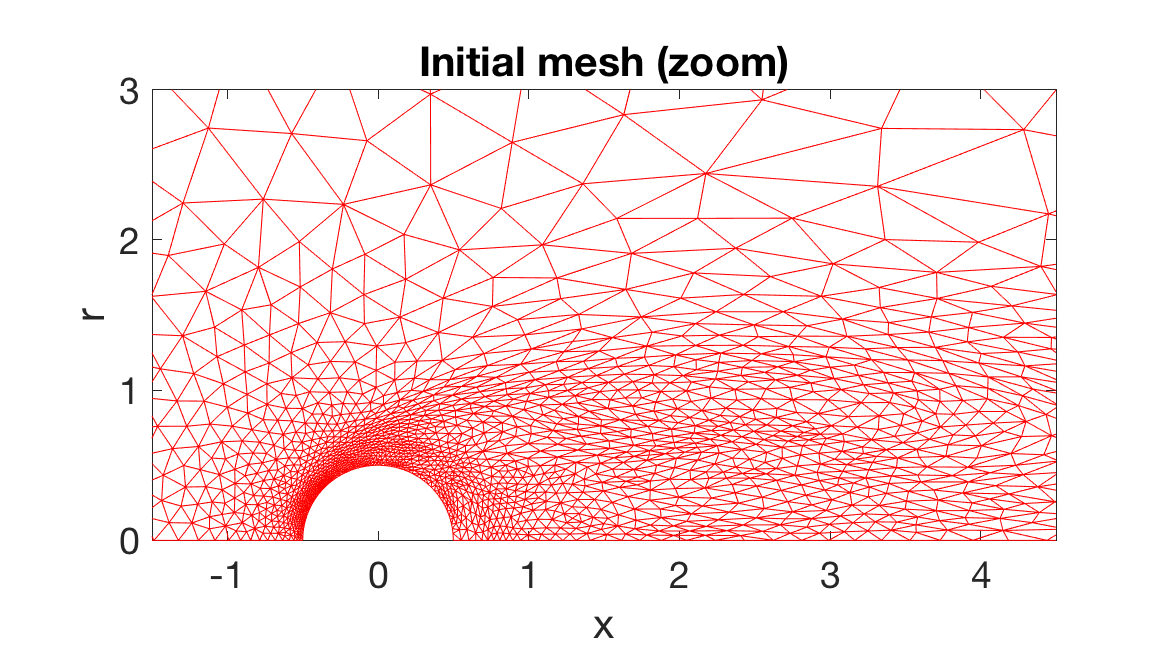
\includegraphics[width=.9 \linewidth]{Cylinder_Mesh.png}
%\vspace{-.5cm}
%\vspace{-.5cm}
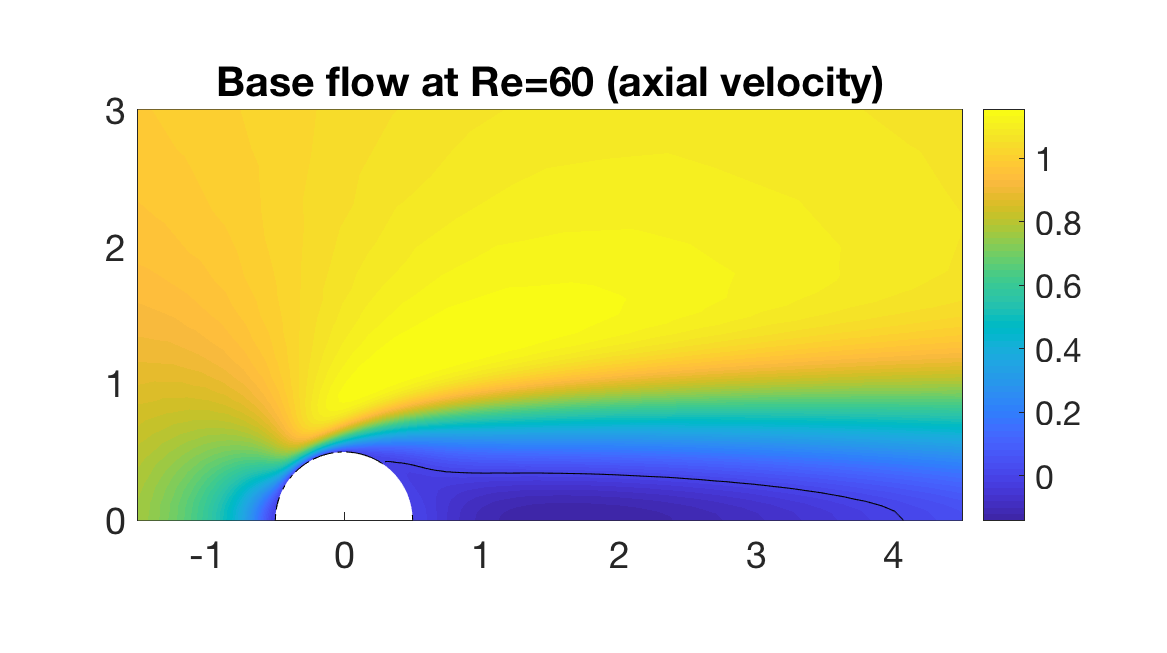
\includegraphics[width=.9 \linewidth]{Cylinder_BaseFlowRe60.png}
%\vspace{-1.cm}
\caption{Adapted mesh $(top)$  and base flow (axial velocity component) ($bottom$) for the flow over a cylinder at $Re=Re_c = 46.7$.}
\label{fig:Baseflow}
\end{figure}

\begin{figure}
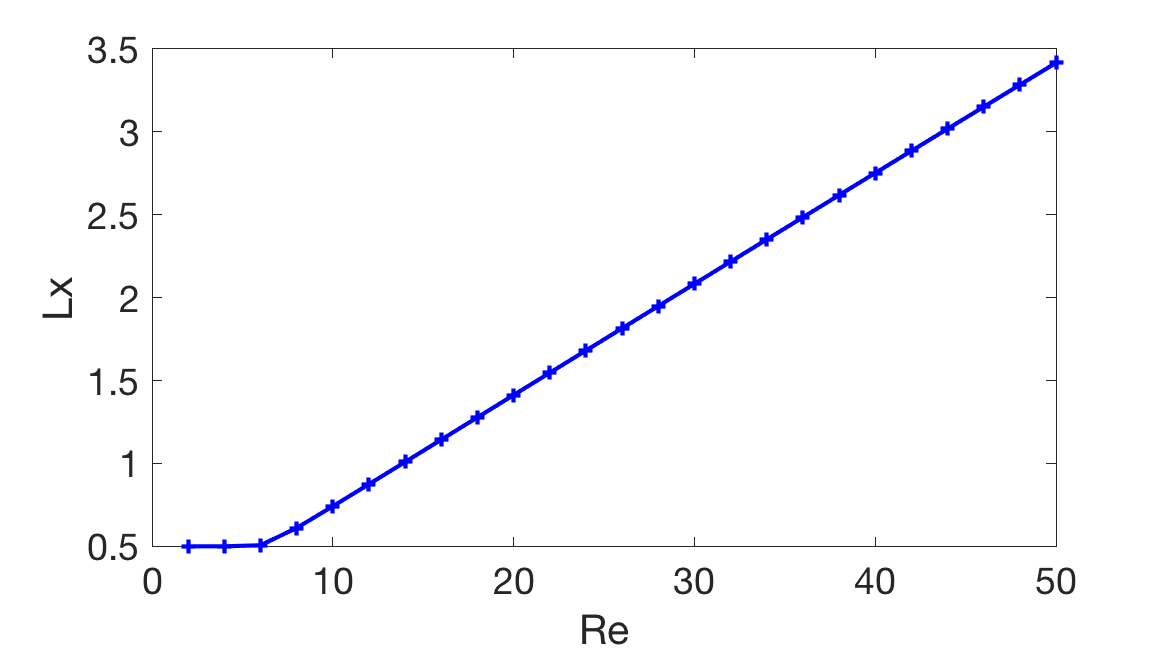
\includegraphics[width=.9 \linewidth]{Cylinder_Lx_baseflow.png}
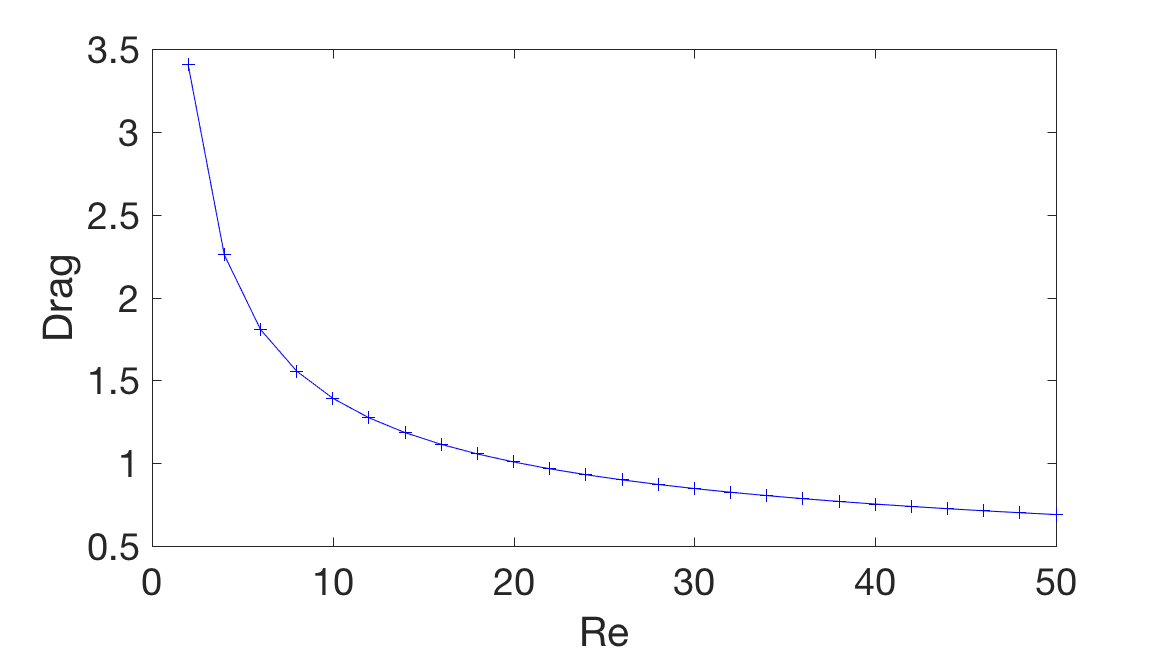
\includegraphics[width=.9 \linewidth]{Cylinder_Drag_baseflow.png}
\caption{Recirculation length $L_x$ $(a)$  and drag $C_x$ ($b$) of the base flow over a cylinder as function of $Re$.}
\label{fig:LxandDrag}
\end{figure}




\subsection{Mesh adaptation procedure}
\vspace{.2cm}

As for any numerical method, a crucial point in the numerical efficiency is the design of the mesh. The finite element method allows to use unstructured mesh and hence to locally adapt the refinement. %Following Sipp \& Lebedev, 
The most common procedure is to decompose the domain into several parts with different grid densities; for instance for the wake of a cylinder, we will design a near-wall region with very small  size, a "wake" region with intermediate mesh size, and an outer region with large mesh size. The inconvenient is that the design relies on an a priori expectation of the regions where gradients will be large. 

In our implementation, we used an automatic mesh adaptation method. %which provides an optimal mesh adapted to the structure of the flow. 
The implementation relies on the AdaptMesh procedure of the FreeFem++ software. This procedure is detailed in detail in ref. \cite{adapt}. 
In short, the classical Delaunay-Voronoi algorithm produces a mesh with gridpoint distribution specified by a {\em Metric } matrix $\cal M$. The AdaptMesh algorithm consists of using as a metric the {\em Hessian} (second-order spatial derivatives) of an objective function $u_h$ defined over the domain, i.e. ${\cal M} = \nabla \nabla u_h$. The precision can be controlled by specifying an objective value for the interpolation error of the function on the new mesh.

To build an optimal mesh for the base-flow calculation, the idea is to use as the objective function $u_h$ the solution ${\bf u}_b$ itself, as computed on a previous mesh.%The procedure thus ensures that the mesh will be locally adapted to the gradients of the base flow. 
The base flow is then recomputed on the adapted mesh, providing a better approximation of the solution. The procedure can be repeated a few steps to ensure a right convergence.

The mesh generated in the previous way may not be optimal for the stability calculations as the structure of the eigenmode may be more complex than that of the base flow. To remedy with this, the idea is to subsequently adapt the mesh to both the mesh flow and the results of the stability calculation. This is easily done with FreeFem, as the  AdaptMesh procedure can be used with several objective functions. We have experimented two different ideas. The first is to adapt the mesh to the base flow and the structure of the leading eigenmode. A second and smarter idea is to adapt the mesh to the base flow and the structural sensitivity. Results show that the two procedures yield the same values for the eigenvalues with less than $1\%$ error, but that the second method gives a mesh with about 3 times less grid points, leading to much faster computations (see appendix A). So, if one is interested only in the eigenvalues, for instance to plot growth rates as function of Reynolds or to identify the critical Reynolds number, mesh adaptation to the sensitivity gives the best option. On the other hand, if one is interested in the detailed structure of the eigenmode, which may extend far away from the wavemaker region, it is advised to use mesh adaptation on the eigenmode. 

In our implementation, the whole process is performed using the Matlab driver {\em Freefem\_AdaptMesh.m} ; the kind of adaptation  (to base flow only, to eigenmode, or to sensitivity) is decided by the choice of parameters transmitted to this function.






\section{Illustration for the wake of a cylinder} 
\vspace{.2cm}

\paragraph{Problem description}
Here, we consider the two-dimensional flow past a circular cylinder. All flow quantities are normalized using 
the uniform incoming velocity $U_{\infty}$ and the cylinder diameter $D$, which are the characteristic velocity and 
length scales used for the definition of Reynolds number $Re= U_{\infty} D / \nu$.
The origin of the cartesian frame of reference is considered located on the cylinder axis, the x-axis is chosen to be parallel to the incoming free-stream velocity while the y-axis with the cross-stream velocity.
The dimensions of the computational domain are the following: $-40 \le x/D \le 80$ and $-40 \le y/D \le 40$.
We impose a no-slip condition $(u=0,v=0)$ on the cylinder surface (${\Gamma_{cil}}$), a uniform velocity $(u=1,v=0)$ at the inflow 
$x/D=-40$ and a no-stress condition at the outlet $x/D=80$ and on the lateral boundaries of the computational domain $y/D=\pm 40$.

%Domain dimension $[-40,80]x[0,40]$. No-stress conditions at outlet AND LATERAL BOUNDARY.
The hydrodynamic loads can be obtained by integrating the stress tensor over the cylinder surface.
In particular, the hydrodynamic lift and drag forces read 

\be{drag}
D = F_x ({\bf u},p) = 
 \int_{\Gamma_{cil}} \left[-p {\bf n} + \frac{2}{Re} {\bf D}({\bf u}) \cdot {\bf n} \right]   \cdot {\bf e_x} d\ell
\ee


\be{lift}
L = F_y ({\bf u},p) = 
 \int_{\Gamma_{cil}} \left[-p {\bf n} + \frac{2}{Re} {\bf D}({\bf u}) \cdot {\bf n} \right]   \cdot {\bf e_y} d\ell. 
\ee



\paragraph{Mesh adaptation procedure}

Let's consider now the matlab code reported in figure \ref{Listing2}. First we build an initial mesh (line 1), and compute base flow solutions for increasing values of the Reynolds number up to $Re = 60$ (lines 3-9).
Then we perform the mesh adaptation with the structural sensitivity, as explained in a previously (line 13). 
The resulting mesh, depicted in figure \ref{fig:Baseflow}, is used for the rest of the computations presented in this paper (except for displaying the eigenmode in figure 4$a$). 
Appendix A presents additional test regarding mesh convergence, and demonstrate that results obtained with the resulting mesh are trustable within $1\%$ accuracy for the eigenvalue, while requiring a very reasonable number of grid points compared to previous studies of this problem. 


%It is shown that as well as doing mesh adaptation with the eigenmode structure instead of the sensitivity, as discussed above, gives comparable results within $1\%$ as for the eigenvalue of the most amplified mode.







%The produced outputs (lines 14-17) gives information about the resulting mesh. 
%Note the values $h_{min}$ and $h_{max}$ of the smaller and larger edges, as well as the local grid size at four points A,B,C,D defined as $(x_A,y_A) = (0.5,0)$ (at the surface of the cylinder at the position of maximum shear), $(x_B,y_B) = (0.5,2.5)$ (at the location of the peak of structural sensitivity, see next section), $(x_C,y_C) = (0.,4)$ (in the near wake), and $(x_D,y_D) = (0.,10)$ (in the the far wake). Finally, the base flow is automatically recomputed on the resulting mesh (line 18-19). Finally, lines 21-22 plot the mesh and base flow structure, producing the result displayed in figure (\ref{fig:Baseflow}).

\paragraph{Base flow}

Having thus produced a convenient mesh, we can now illustrate the properties of the base flow as function of Reynolds number. Figure \ref{Listing2} shows how to compute and plot with StabFem the two most commonly studied quantities, namely the recirculation length $Lx(Re)$, i.e. the location of the stagnation point at the rear of the recirculation region, and the drag coefficient $C_x(Re)$.
Note that the object \verb|bf| is defined as a structure with fields \verb|Drag| and \verb|Lx|. 
The resulting plots are given in figure \ref{fig:LxandDrag}, and are in good agreement with known results for this classical problem.
In particular, for low Reynolds, the recirculation $L_x(Re)$ is equal to $0.5$ (which is the radius of the cylinder) indicating the absence of a recirculation region. The latter appears for $Re > 4.8$, in accordance with known results.




%\subsection{Implementation}

%\subsection{Application to the cylinder}


%\clearpage

%We now review the main concepts of linear stability approach and explain how such calculations are implemented in our software.

\begin{figure}
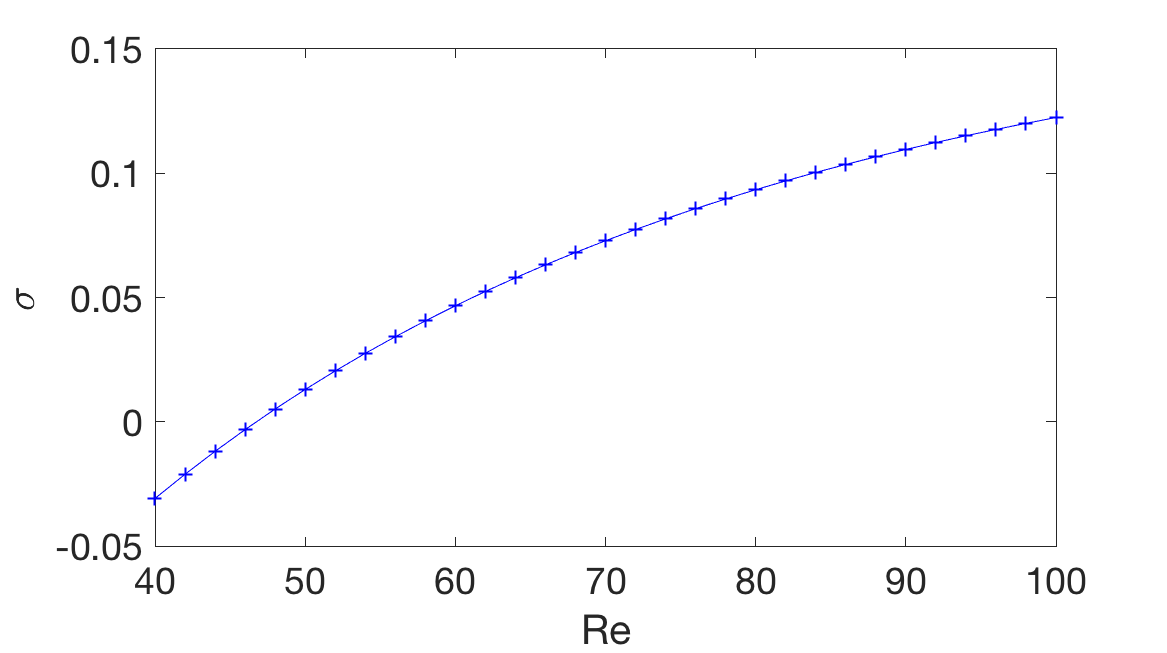
\includegraphics[width=.9 \linewidth]{Cylinder_Sigma_Re.png}
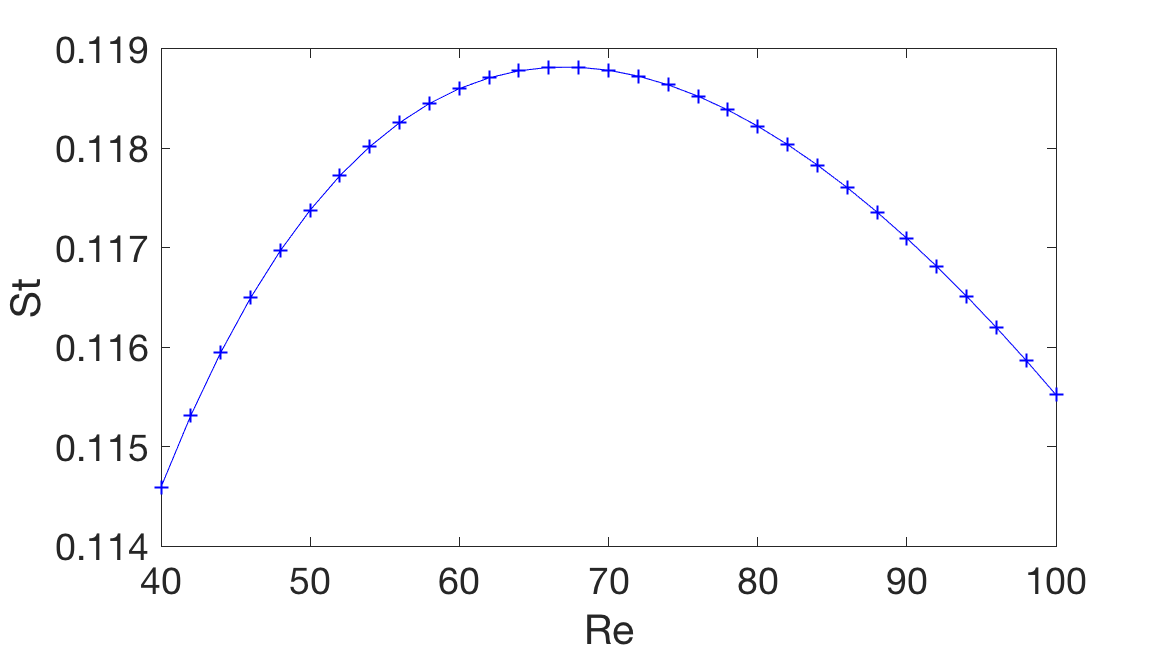
\includegraphics[width=.9 \linewidth]{Cylinder_Strouhal_Re.png}
\caption{Growth rate $\sigma$ $(a)$  and Strouhal number $St = (a \omega)/(2\pi U_{\infty})$ ($b$) as function of Reynolds number}
\label{fig:SigmaOmega}
\end{figure}

\begin{figure}
%\vspace{-.5cm}
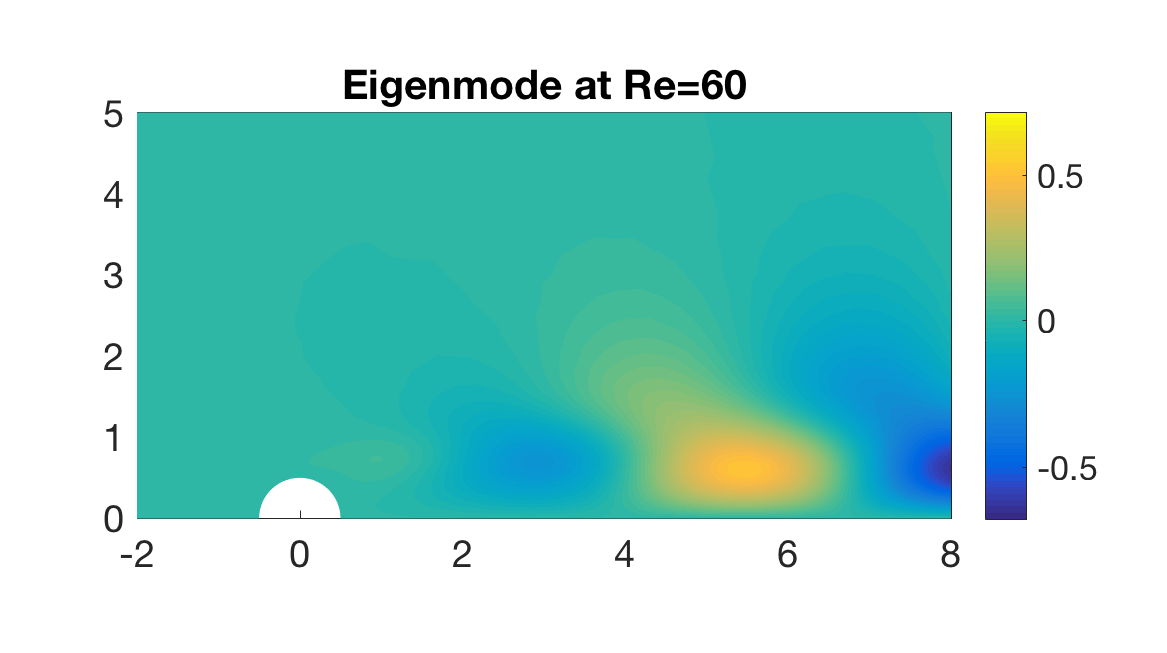
\includegraphics[width=.9 \linewidth]{Cylinder_EigenModeRe60.png}
%\vspace{-.5cm}
%\vspace{-.5cm}
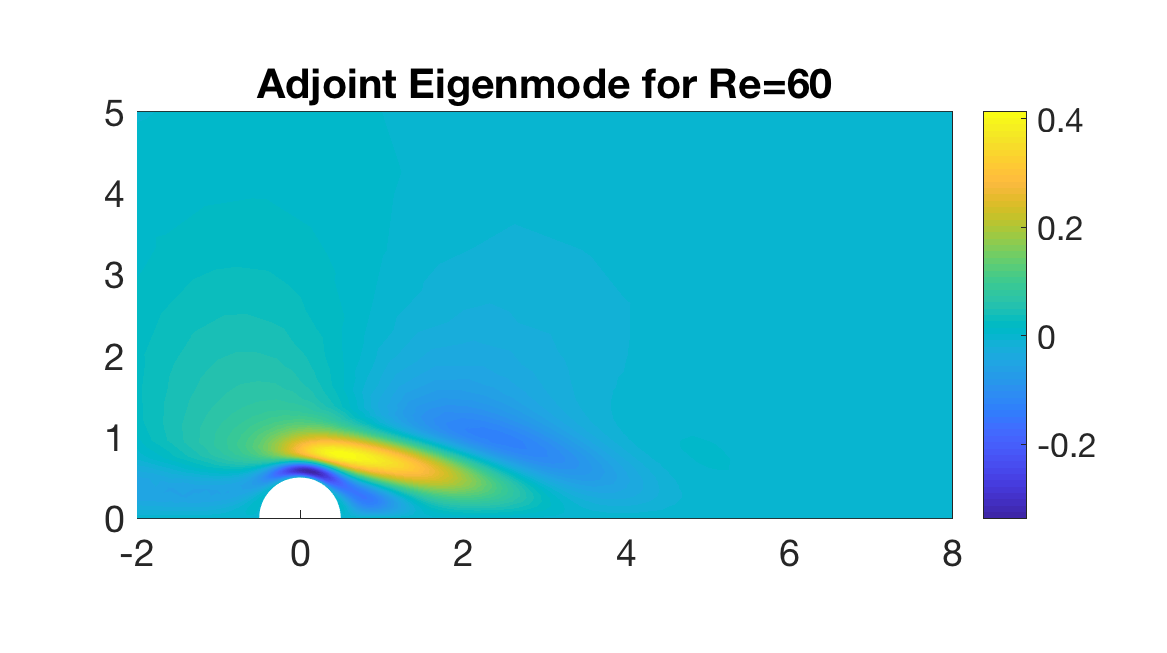
\includegraphics[width=.9 \linewidth]{Cylinder_EigenModeAdjRe60.png}
%\vspace{-.5cm}\vspace{-.5cm}
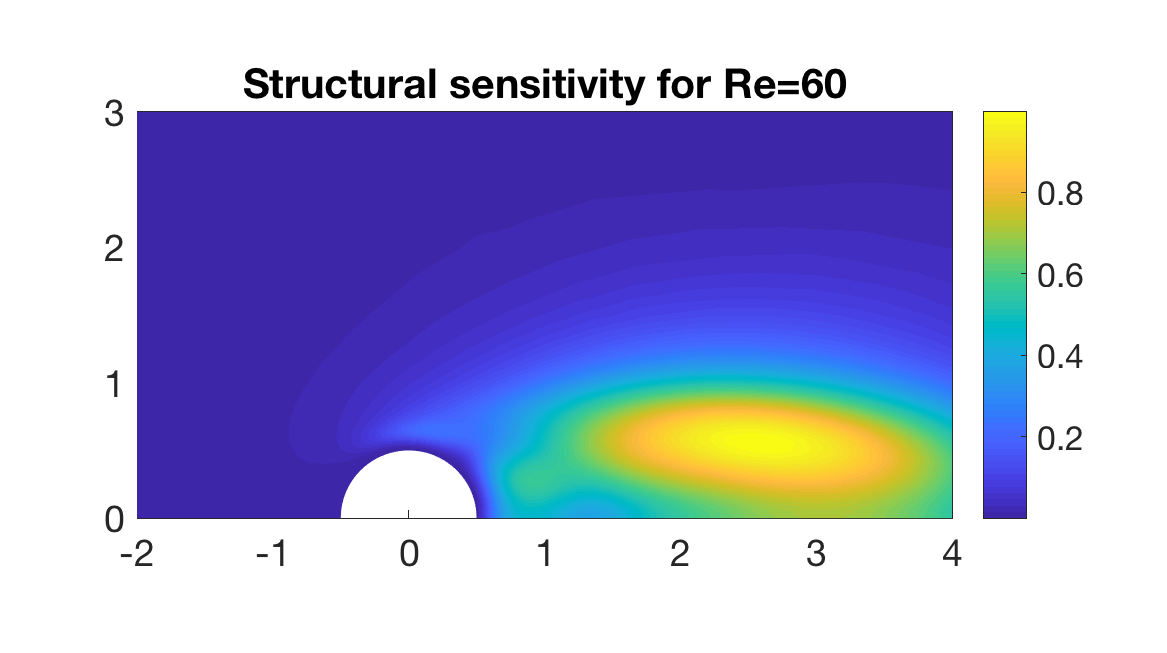
\includegraphics[width=.9 \linewidth]{Cylinder_SensitivityRe60.png}
%\vspace{-.5cm}
\caption{Contour plot of the streamwise velocity component: $(a)$ (Direct) Eigenmode; $(b)$ Adjoint mode and ($c$) Structural sensitivity field for the cylinder's wake at $Re=Re_c = 46.7$.}
\label{fig:Eigenmode}
\end{figure}


%\begin{figure*}
%\small
%\begin{lstlisting}
%\end{lstlisting}
%\normalsize
%\caption{Illustration of the procedure to compute stability properties and adapt the mesh using StabFem (from script {\em SCRIPT\_CYLINDER.m}. }
%\label{listing4}
%\end{figure*}

\paragraph{Linear stability results}

We investigate the stability of the base flow fields by performing a parametric study of the eigenproblem 
(\ref{Eigen_matricial}). In this way, we determine the critical Reynolds number $Re_c$ at with the steady base flow
first becomes unstable: to this end it is useful to remember that a flow state is 
linearly unstable when the real part of 
the leading eigenvalue, i.e. the growth rate, is positive. 
Figure \ref{fig:SigmaOmega} shows growth rate and the Strouhal number 
$St=a\omega/2 \pi U_{\infty}$ as a function of the 
Reynolds number. It is easy to check that the critical Reynolds number is about 47 
for the first mode. 
The associated direct eigenmode is depicted in figure \ref{fig:Eigenmode}. The 
spatial structure of this mode 
extends downstream of the bluff body and is characterized by streamwise 
extended spatial disturbances. 
On the other hand, the adjoint mode is highly localized near the cylinder 
on the upper (and lower) side of the body surface. 
We recall that the adjoint field provides useful information about the mechanism to
flow receptivity to momentum forcing and mass injection.
We note also that this receptivity decays rapidly both upstream and downstream 
of the bluff body.

The structural sensitivity field displayed in figure \ref{fig:Eigenmode}c)
is obtained by evaluating eq. \ref{Structursens}.
In particular, we plot the spectral norm of the sensitivity tensor, it 
gives the maximum possible coupling among the velocity components. 
This spatial map can be used to identify the flow region where the 
instability mechanism acts.


\section{Nonlinear global stability approaches}
\vspace{.2cm}
%\section{Computing the limit cycle for $Re>Re_c$ with Harmonic Balance}


%For $Re\right>Re_c$, the linear stability analysis based on the {\em base flow} does not allow to predict the properties of the limit cycle; in particular the Strouhal number is substantially underestimated. %It has been shown that investigating the stability properties of the {\em mean flow} obtained by averaging time-marching solution gives a better accordance. Attempts to on a rigourous basis  
In the past decade, efforts have been devoted to extend the range of validity of global approaches into the nonlinear regime for $Re>Re_c$, with the double objective to describe the properties of the limit cycle reached after saturation and to derive amplitude equations describing the transitent dynamics towards this cycle. The two main milestones in this direction {\color{red} are} the {\em weakly nonlinear model}  (WNL) of Sipp \& Lebedev \cite{SippLebedev} and the {\em self-consistent model} (SC) of Manti\v{c}-Lugo et al \cite{MLugo2014}.
 {\color{blue} In this review, we will address only the first of the two questions, namely {\color{red} the} description of the saturated cycle, and leave aside the question of transient dynamics. We will successively review the two aforementioned models, in a simplified formulation devoted to describe only the saturated cycle. We also provide a simple implementation of these two models. Finally, in line with the previous section, we will again illustrate with results obtained for the wake of a cylinder.
 }
 
 

\paragraph{General definitions in the nonlinear r{\color{red}e}gime}
 
In this part, to simplify the notations, we symbolically write the Navier-Stokes equations, as {\color{red}$\partial_t {\bf u} = {\cal NS} ({\bf u})$}, therefore dropping the systematic reference to the incompressibility constraint and associated pressure field. 

In the nonlinear r{\color{red}e}gime, the {\em base flow} introduced in the linear theory is not directly accessible and no longer relevant, especially when the oscillation amplitudes become large. 
Instead, {\color{red} we taken the decomposition ${\bf q}={\bf q}_m({\bf x})+{\bf q}'({\bf x},t)$, with ${\bf q}'$ the nonlinear perturbation and ${\bf u}_m$ the {\em mean flow} defined as the time-average  of the flow:}
\be{defumean}
{\bf u}_m({\bf x})  = \frac{1}{T} \int_0^{T}  {\bf u}({\bf x},t)  dt,
\ee
where $T = 2\pi/\omega$  is the period of the oscillation cycle.

A convenient measure of the unsteady part of the flow, which has been adopted in both the WNL and SC models, is the energy-amplitude, defined as the square-root of the total energy associated to the fluctuating part of the velocity field:
\be{defAnergy}
A_E = \sqrt{\frac{1}{T} \int_0^{T} \left( \int_\Omega | {\bf u} - {\bf u}_m |^2 \, dS \right) dt}.
\ee

Another quantity which has been particularly addressed in previous studies is the mean recirculation length $L_x$
already discussed{\color{red},} introduced and documented in figure {\color{red}??}. {\color{red} However, in a} nonlinear regime, the recirculation bubble becomes unsteady, {\color{red} becoming} difficult to define properly an instantaneous recirculation length. It is still possible to define a mean recirculation length associated to the mean flow. %On va le faire ??

In the next sections we will document the predictions of the WNL and SC models regarding the quantities $A_E$ and $L_x$ adopted in past studies. In addition, we will document two other quantities of practical interest : the Drag and Lift forces $F_x$ and $F_y$ exerted on the cylinder. 
Both are periodic functions of time and{\color{red},} owing to symmetry consideration, the drag contains only even harmonics and the lift only odd harmonics:{\color{red}
\be{drag_lift_def}
\begin{cases}
F_x=F_{x,0} + \sum_{n=1}^\infty \big( F_{x,2n,c} \cos ( 2 n \omega t) + F_{x,2n,s} \sin( 2 n  \omega t ) \big) \\
\begin{split}
F_y  =  \sum_{n=1}^\infty \big(  F_{y,{2n-1},c} \cos ((2n-1) \omega t ) +\\
 F_{y,(2n-1),s} \sin ((2n-1) \omega t) \big)
\end{split}
\end{cases}.
\ee
}
In the sequel we will focus on the {\em mean drag}  $F_{x,0}$ and on the fundamental frequency part of the lift given by $F_{y,1,c}$ and $F_{y,1,s}$.
 
   
%MThe mean drag is given by 

%$$F_{x,m} = D(u_m)$$
%with "Drag" operator defined in equation ().

%The oscillating lift $F_y(t)$  is a	 periodic function of period $T$, and we will 
%$$F_y = F_y,c


%The first milestone in this direction is the work of Sipp \& Lebedev \cite{SippLebedev} who used a weakly nonlinear development in terms of the distance to the threshold $Re-Re_c$. However, although derived on rigorous grounds, the weakly nonlinear development has a very limited range of validity and already fails for $(Re-Re_c) \approx 1$.
%More recently,  Manti\v{c}-Lugo et al \cite{MLugo2014} proposed an alternative approach termed {\em Self-consistent model} which succeeds in predicting the dynamics up to $Re =120$ and more. 
%This model was build as a linear stability approach build on a {\em mean flow} which includes a retroaction of the eigenmode. However, if one is interested in the limit cycle and not the transient,
%the approach is actually equivalent to a Fourier series decomposition of the flow with respect to time (an approach also known as {\em harmonic balance}) retaining only the two first terms. 
%The approach is based on a generalisation of the eigenmode ansatz \ref{} and 

%In the next sections, we thus successively present the weakly nonlinear model, the self-consistent model, and propose a direct resolution method for this latter model. 


%The relation with the initial method of Mantic-Lugo et al. will be discussed afterwards.


\paragraph{Weakly nonlinear model}
%REFAIRE
\begin{figure*}
\small
\begin{lstlisting}
[bf,em]=SF_FindThreshold(bf,em);
wnl = SF_WNL(bf,em);

Re_HB = [Rec 47.5 48 49 50 55 60 65 70 75 80 85 90 95 100];
omega_HB = [Omegac]; Aenergy_HB = [0]; 

bf=SF_BaseFlow(bf,47.5);
[ev,em] = SF_Stability(bf,'shift',Omegac*i);
Astart = sqrt(wnl.Lambda/(wnl.Nu0+wnl.Nu2)*(1/Rec-1/47.5));
[meanflow,mode] = SF_HarmonicBalance(bf,em,'sigma',0.,'Re',47.5,'Aguess',Astart);

for Re = Re_HB(2:end)
    [meanflow,mode] = SF_HarmonicBalance(meanflow,mode,'Re',Re);
    omega_HB = [omega_HB imag(mode.lambda)];
    Aenergy_HB  = [Aenergy_HB mode.Energy];
end

\end{lstlisting}
\normalsize
\caption{Illustration of the procedure for nonlinear calculations using StabFem (from script {\em SCRIPT\_CYLINDER.m}. }
\label{fig:listingNL}
\end{figure*}

We give here a brief account of the weakly nonlinear model of Sipp \& 
Lebedev\cite{SippLebedev}, also discussed by Gallaire et al. \cite{FDR2016}. 
The derivation is based on a multiple scale  decomposition based on the parameter {\color{red}$\epsilon^2 = 1/Re_c - 1/Re$}. 
In the case where we are interested only in the desciption of the saturation cycle, the starting point can be taken as the following expansion of the state-vector ${\bf{q}}=({\bf{u}},p)$ defining the flow:
\be{WNL1}
\begin{aligned}
&{\bf q} = {}  {\bf q}_{bc} + \epsilon \left[ A_{wnl}  \hat{\bf q} e^{i (\omega_c+\epsilon^{\color{red}2} \omega_\epsilon)  t} + c.c. \right]\\
&+ \epsilon^2 \left[ {\bf q}_\epsilon + |A_{wnl}|^2  {\bf q}_{2,0} + \left(  A_{wnl}^2 {\bf q}_{2,2} e^{2 i(\omega_c+\epsilon^{\color{red}2} \omega_\epsilon)  t} + c.c. \right) \right]\\
& + {\cal O}( \epsilon ^3),
\end{aligned}
\ee
where ${\bf q}_{bc}$ is the base flow at the threshold $Re_c$, $\hat{\bf q}$ the neutral 
eigenmode at $Re_c$, {\color{red} $A_{wnl}$ an amplitude,} $\omega_c$ the frequency predicted by the linear approach at $Re=Re_c$ and $\omega_\epsilon$ a small deviation of the frequency, {\color{red} ${\bf q}_{\epsilon}$ the base flow modifications related to the increase of $\epsilon$, ${\bf q}_{2,0}$ the flow response to the steady nonlinear interactions of $\hat{\bf q}$ with its conjugate, ${\bf q}_{2,2}$ the flow response to the unsteady nonlinear interactions of $\hat{\bf q}$ with itself and  ${\cal O}( \epsilon ^3)$ the third order terms.   }

Note that this starting point is slightly different from the original approach of \cite{SippLebedev} who used a multiple scale method and assumed a dependence of the amplitude $A_{wnl}$ as function of a slow time-scale $\tau = \epsilon t$. This latter starting point is the {\color{red}right} way to parametrize the problem if one wants to obtain an amplitude equation, but{\color{red},} as specified above{\color{red},} our goal here is to provide a simpler formulation {\color{red}describing} only the saturated cycle. 

%%%%%%%%%%%%%%%%%%%%%%%%%%%%%%%%%%%%%%%%%%%%%%%%%%%%%%%%%%%
%%%%%%%%%%%%%%%%%%%%%%%%%%%%%%%%%%%%%%%%%%%%%%%%%%%%%%%%%%%
%DETAILS IN APPENDIX
%%%%%%%%%%%%%%%%%%%%%%%%%%%%%%%%%%%%%%%%%%%%%%%%%%%%%%%%%%%
%%%%%%%%%%%%%%%%%%%%%%%%%%%%%%%%%%%%%%%%%%%%%%%%%%%%%%%%%%%
%%%%%%%%%%%%%%%%%%%%%%%%%%%%%%%%%%%%%%%%%%%%%%%%%%%%%%%%%%%
{\color{red}
The expansion \ref{WNL1} can be introduced into the Navier-Stokes equations \ref{NSprimitive}. Details at the different $\epsilon^i$ orders are given in the appendix}. The outcome is a relationship with the form
\be{WNL3}
i \omega_\epsilon A_{wnl} = \Lambda A_{wnl} - (\nu_0+\nu_2)  |A_{wnl}|^2 A_{wnl},
\ee
where the coefficients $\Lambda$, $\nu_0$ and $\nu_2$ are given by {\color{red}equations \ref{LAMBDA}, \ref{NU0} and \ref{NU2}, respectively.

We note that $\Lambda$ does not depend on the normalization choice of the eigenmode, discussed later, while $\nu_0$ and $\nu_2$ depend. Hence, if one is interested in the amplitude of the limit cycle, the latter will depend on it and will be given by $|A_{wnl}| = \sqrt{\Lambda_r/(\nu_{0,r}+\nu_{2,r})}$.

Reintroducing the scaling
\be{ANL} 
|A| =  \epsilon |A_{wnl}| =\sqrt{ \frac{\Lambda_r}{\nu_{0,r}+\nu_{2,r} }} \sqrt{\frac{1}{Re_c}-\frac{1}{Re}},
\ee
the frequency of the limit cycle is given by
\be{omegaWNL} 
\omega_{LC}=\omega_c+ \epsilon^2\Lambda_i- (\nu_{0,i}+\nu_{2,i})|A|^2.
\ee 
}
{\color{red}

Recasting equation \ref{WNL1} in the {\em mean flow} definition \ref{defumean}, we obtain
\be{mean_flow_WNL}
{\bf u}_m({\bf x })= {\bf u}_{bc}+\epsilon^2 {\bf u}_\epsilon + |A|^2{\bf u}_{2,0},
\ee
where the first two terms give the base flow approximation at the $Re$ prescribed by $\epsilon$. }

The associated Drag and Lift are given respectively by:
\begin{eqnarray}
F_{x,WNL} &=& F_{x}({\bf q}_{bc})+\epsilon^2 F_{x}({\bf q}_{\epsilon})+F_{x}({\bf q}_{2,0})|A|^2,\\
F_{y,WNL} &=& |A|^2 \big[ F_{y}({\bf \hat{q}})e^{i\omega_{LC} t} +c.c. \big],
\end{eqnarray}
where $F_{x}$ and $F_{y}$ are given by \ref{drag} and \ref{lift}, respectively.


I'M HERE


{\color{blue}
A key issue in the weakly nonlinear expansion is that the definition of the amplitude depends upon a normalization choice 
of the eigenmodes. Several choices are possible. In the litterature three possibilities have been used :
\begin{itemize}
\item First, \cite{SippLebedev} normalized the eigenmode by assuming a specified value to the $y$-component of the velocity at one point, namely :
\be{normsipp}
\hat{u_y}(1,0) = 0.4612
\ee
The advantage of this choice is that the amplitude is then a measure of the energy of the perturbation: 
$\epsilon A_{wnl} \approx A_E$.

\item Secondly, \cite{FDR2016} proposed the following normalisation choice :
\be{normFDR}
\int_\Omega |\hat{\bf u}|^2 d {\bf x}  = \frac{1}{2}
\ee
This directly leads to $\epsilon A_{wnl} = A_E$.

\item Thirdly, following \cite{Fabre2012}, another convenient choice is to normalize the eigenmode with its lift 
force : 
\be{normfabre}
L(\hat{\bf u};\hat{p}) = 1/2
\ee
The advantage of this choice is that the amplitude $\epsilon A_{wnl}$ is directly related to the fundamental lift :
$
F_{y,1,c} 
%= \epsilon A \left( 1/2 e^{i \omega t} + c.c. \right)
=   \epsilon A \cos (\omega t) ; \quad F_{y,1,c} = 0. 
$

\end{itemize}
}

In our implementation of the WNL approach, we allowed to choose the normalization convention. 
In table (??) we give the predictions of the WNL approach using the three normalization choices.
We can note that the coefficients $\nu_0$ and $\nu_2$ strongly depend on the normalization choice.
on the other hand, the frequency deviation as well as the drag and lift coefficients are independent of it.
 


\begin{table}
$$\begin{array}{cc}
a&b
\end{array}$$
\caption{Coefficients of the weakly nonlinear coefficients : }
\end{table}




Figure \ref{fig:listingNL}, which is extracted from the script 
\verb|SCRIPT_CYLINDER_DEMO.m|, illustrate the sequence of commands to 
perform the weakly nonlinear study for the cylinder wake.
On line 1, we first determine the instability threshold, and the corresponding base flow 
and eigenmode\footnote{This routine uses Newton iteration to directly compute the 
base flow, the eigenmode, the frequency and the critical Reynolds. The algorithm is 
very similar to the one presented for the HB, with an additional unknown (Re) and an 
additional constraint (normalization of the mode). The interested reader should 
reconstruct easily the whole procedure from the code provided.}.
On line 2, we then compute all the terms and coefficients of the WNL model. 
%After that, 
%we construct  vectors to store the frequency and the amplitude of the limit cycle in the 
%range $Re = [47.5-100]$. Note that for the computation at $Re=47.5$, we need a guess 
%for the amplitude, which is deduced from the weakly nonlinear approach on line 9. In 
%the sequel of the loop no guess value is prescribed, hence the solver uses 
%continuation.



As can be seen on figure \ref{fig:Comp2},  the approach gives good prediction in the immediate vicinity of $Re_c$, but deviation appears very rapidly and disagreement is already large at $Re=48$ (although, as discussed by Gallaire et al.? and also observed by Tchoufag et al. \cite{Tchoufag2015}, a convenient definition of the $\epsilon$ improves the results).

\begin{figure}
\begin{center}
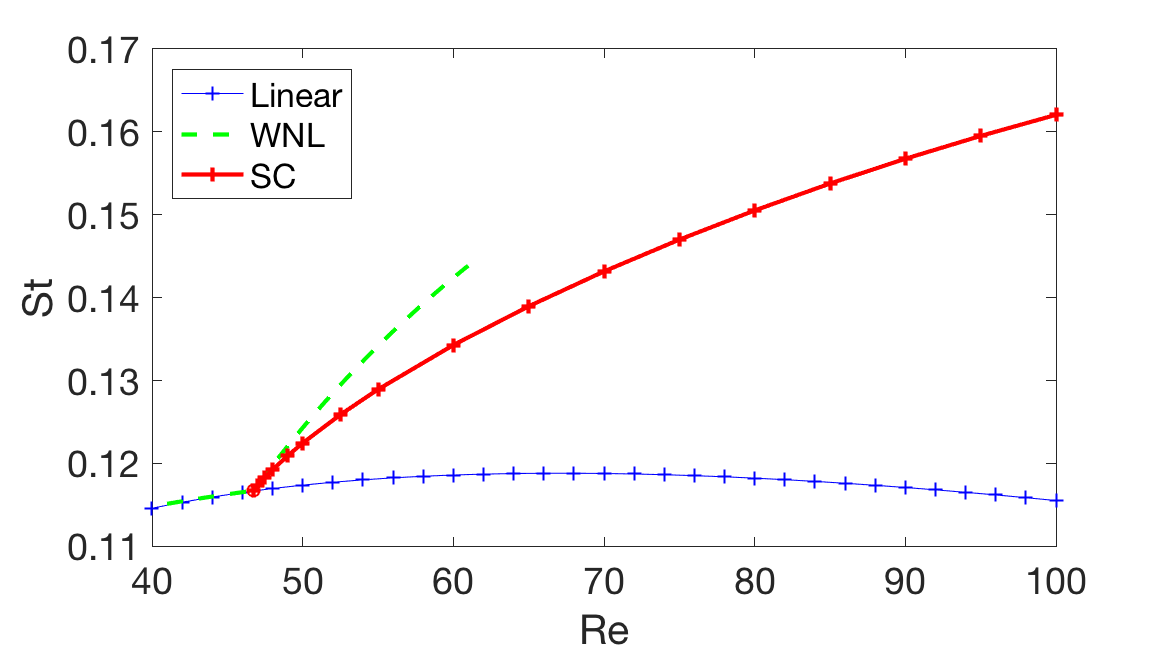
\includegraphics[width=.9 \linewidth]{Cylinder_Strouhal_Re_HB.png}
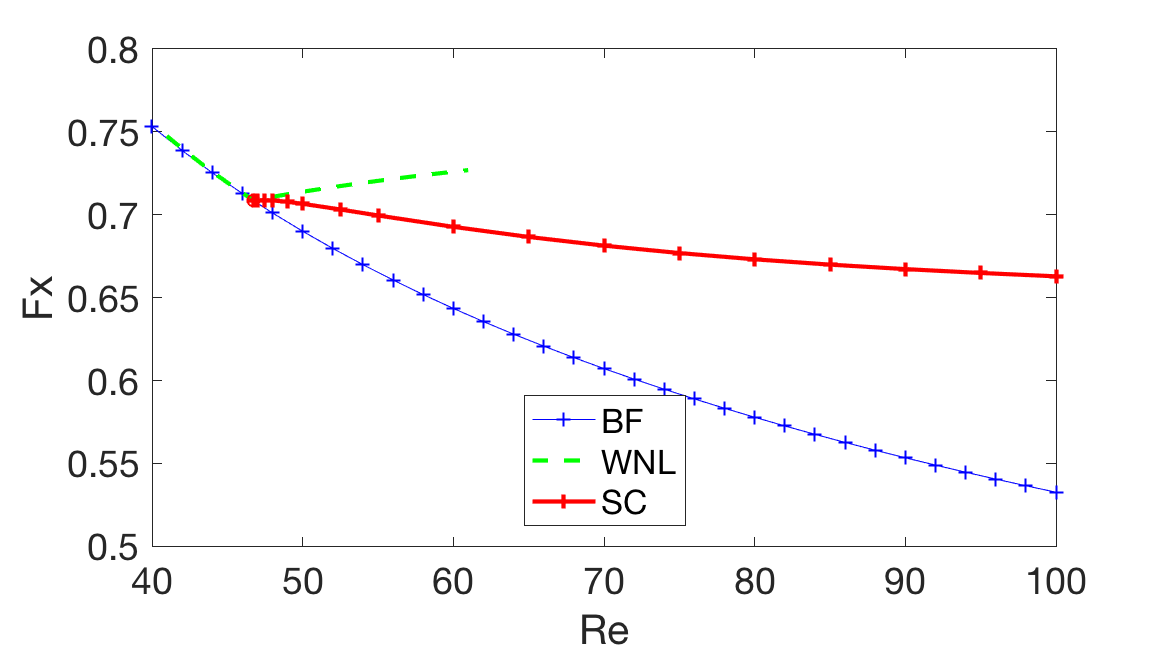
\includegraphics[width=.9 \linewidth]{Cylinder_Cx_Re_HB.png}
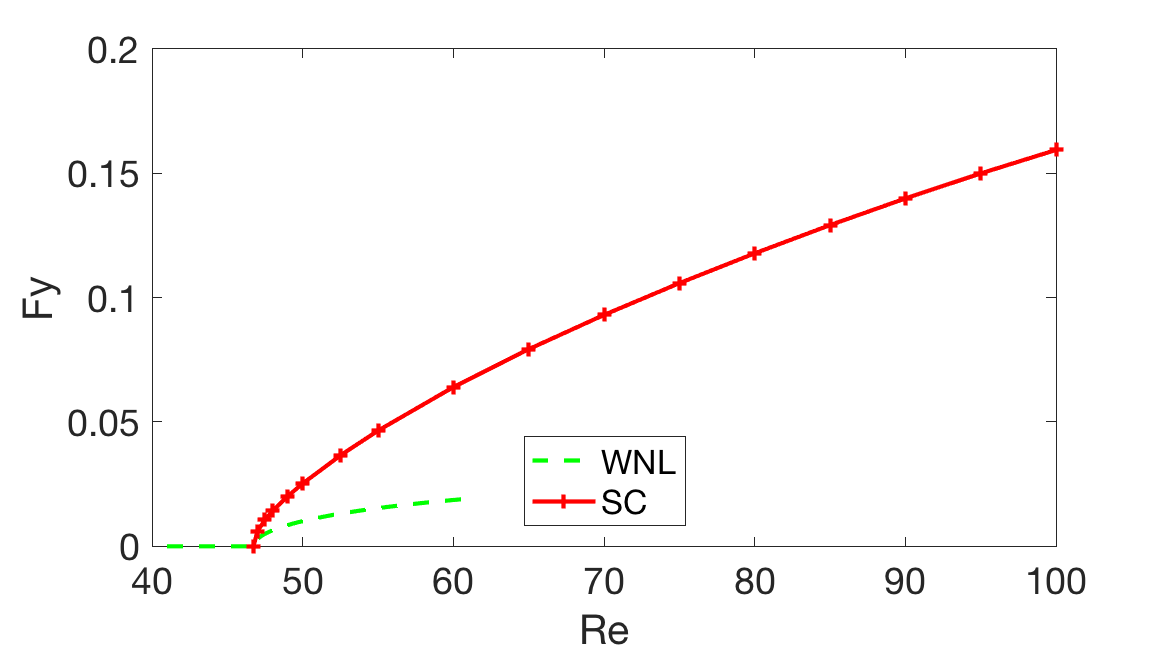
\includegraphics[width=.9 \linewidth]{Cylinder_Cy_Re_SC.png}
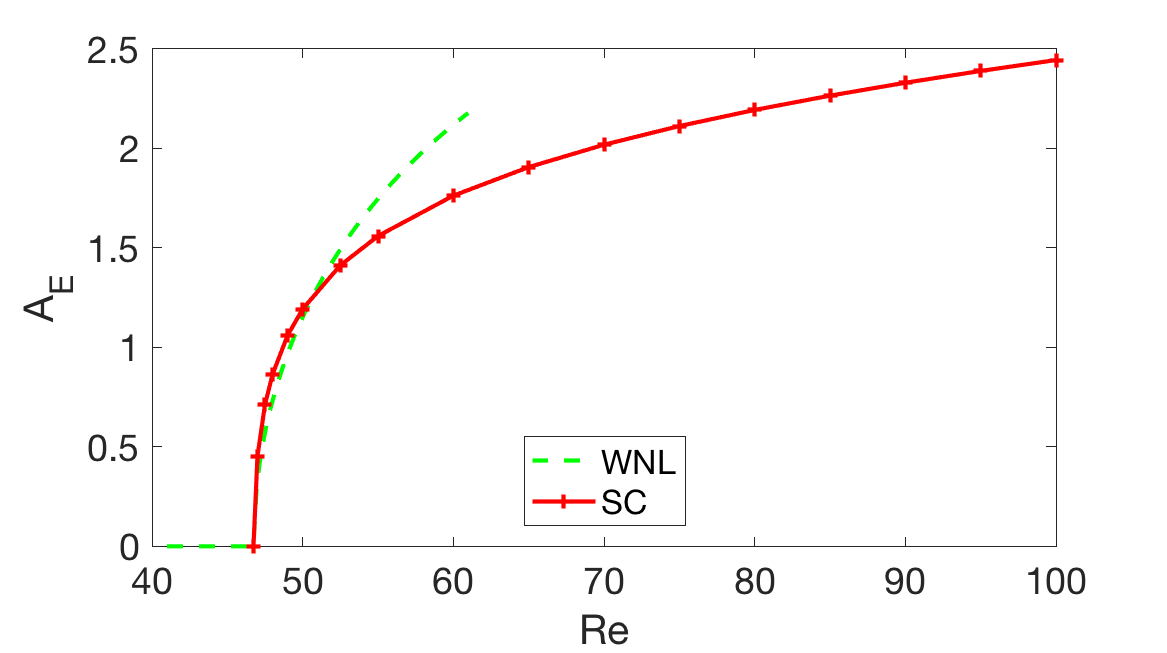
\includegraphics[width=.9 \linewidth]{Cylinder_Energy_Re_SC.png}
\end{center}
\caption{Comparison between the weakly nonlinear results (WNL) and the harmonic 
balance data (HB). We report also the Strouhal number computed by using the 
classical linear stability theory (Linear) and the base flow (BF) $C_x$.
%c_x should be consistent with the drag definition given at beginning
}
\label{fig:Comp2}
\end{figure}


\paragraph{Self-Consistent approach}

TO BE SHORTENED

%\begin{figure}
%\begin{center}
%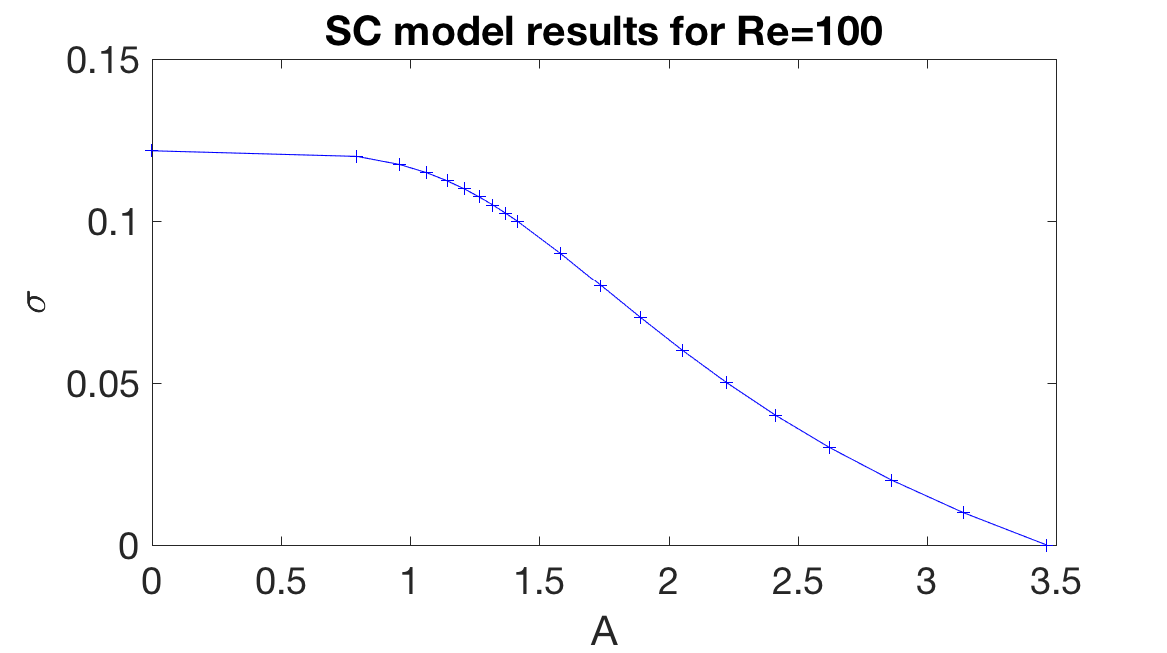
\includegraphics[width=.9 \linewidth]{Cylinder_SC100_EnergySigma.png}
%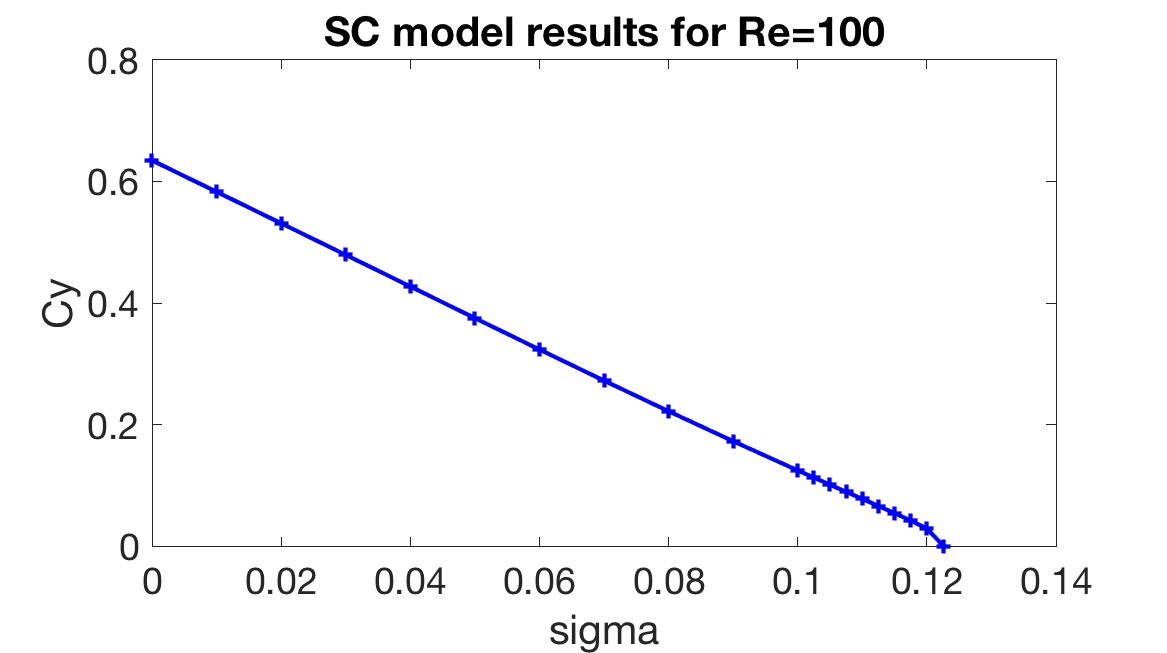
\includegraphics[width=.9 \linewidth]{Cylinder_SC100_CySigma.png}
%\end{center}
%\caption{Self-consistent approach for the wake of a cyrcular cilinder: results at $Re =  100$.}
%\label{fig:SC100}
%\end{figure}

\begin{figure}
\begin{center}
\includegraphics[width=.9 \linewidth]{toto.png}
\end{center}
\caption{Self-consistent approach for the wake of a circular cilinder:  description of the MEAN FLOW for  $Re = 
100$.}
\label{fig:MF60}
\end{figure}


We now briefly review the self-consistent approach as introduced by Manti\v{c}-Lugo et 
al \cite{MLugo2014}. The authors adopted a pseudo-eigenmode expansion of the flow 
as follows: 
\be{SC}
{\bf u } = {\bf u }_m + A_{sc} \left[ \tilde{{\bf u }}_1 e^{\sigma_{sc} t + i \omega_{sc} t} +   \tilde{\bf u }_{-1} e^{\sigma_{sc} t  -i \omega_{sc} t} \right],
\ee  
where ${\bf u }_m$ is the {\em mean flow} defined by phase-averaging over the cycle, $\tilde{{\bf u }}_1$ is a pseudo-eigenvector which is normalized by the condition  $||\tilde{{\bf u }}_1|| = 1/\sqrt{2}$, 
$A_{sc}$ is an amplitude parameter directly related to the energy of the oscillating flow, and $\lambda_{sc} = \sigma_{sc} + i \omega_{sc}$ is a pseudo-eigenvalue which depends upon the parameter $A_{sc}$. 
Introducing the decomposition (\ref{SC}) into the Navier-Stokes equations we are left 
with the following problem:

\begin{subequations}\label{sc12}
\begin{eqnarray}
{\cal NS}(  {\bf u }_m ) - A_{sc}^2 {\cal C}( \tilde{{\bf u }}, \overline{\tilde{\bf u }}) = 0, 
\label{sis1}
\\
(\sigma_{sc} + i \omega_{sc}) \tilde{{\bf u }} =  {\cal L}_{{\bf u }_m}(  \tilde{{\bf u }} ).
\label{sis2}
\end{eqnarray}
\end{subequations}

Equation (\ref{sis1}) provides the mean flow field ${\bf u }_m$ while the 
pseudo-eigenpairs $(\lambda_{sc}, \tilde{{\bf u }})$ can be computed by solving the eigenvalue problem (\ref{sis2}).
%The computed mode is normalized as $ || \tilde{{\bf u }}|| = 1/{\sqrt{2}}$
%is of the same form as  (\ref{HBEq1}) except that $i \omega$ is 
%replaced by $\sigma_{SC} + i \omega_{SC}$. 
% The mean flow is then governed by the same equation
%\ref{HBEq0}) written above, while $\tilde{{\bf u }}_1$ is the solution of an eigenvalue problem with the same form as  (\ref{HBEq1}) except that $i \omega$ is replaced by $\sigma_{SC} + i \omega_{SC}$.

The self-consistent model has the following properties :
\begin{itemize}
\item[-] For $A \ll 1$ it is equivalent to the linear eigenvalue problem (\ref{LEP}), and the generalized eigenvalue coincides with the one predicted by linear stability : $\sigma_{SC} + i \omega_{SC} = \sigma_{lin} + i \omega_{lin}$.
\item[-] For $\sigma_{SC}=0$ (corresponding to a specific choice of the amplitude $A=A_c$),  the expansion (\ref{SC}) is equivalent to a Fourier decomposition of the limit cycle with only two term retained.
\item[-] For $0<A<A_c$, the resolution leads to a relation $\sigma_{SC}(A) ; \omega_{SC}(A)$
such that $0< \sigma_{SC}(A) < \sigma_{lin}$.
 Although in this case the expansion ({\ref{SC}}) cannot represent the flow for all $t$, Manti\v{c}-Lugo et al \cite{MLugo2014} argued that the relation between $\sigma_{SC}$ and $A$ can be used to build an amplitude equation which captures the transient approach to the limit cycle. 
\end{itemize}

Figure \ref{fig:SC100} shows the results of the self-consistent model at Re=100.

\paragraph{Harmonic balance : equations and procedure }

TO BE SIMPLIFIED...

\begin{figure}
\begin{center}
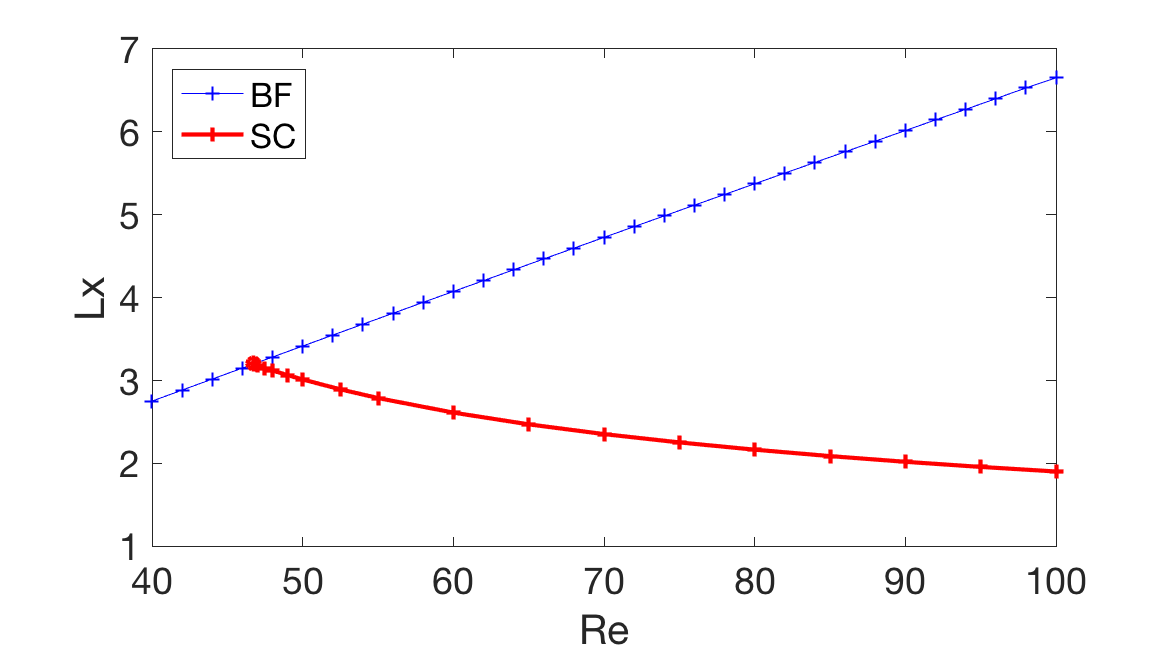
\includegraphics[width=.9 \linewidth]{Cylinder_Lx_Re_HB.png}
\end{center}
\caption{Flow past a circular cylinder: length of the wake bubble (measured from the 
rear stagnation point) for different Reynolds number. Comparison between the base flow bubble and the mean flow bubble computed by using the harmonic balance.}
\label{fig:Comp1}
\end{figure}
As discussed above, the Self-Consistent model was initially presented by the authors as a rational way to explain the dynamics in terms of a stability analysis of the {\em mean flow}. Furthermore, the resolution method presented by the authors, which involves a double iteration loop, is not easy to implement and not particularly efficient.

If one is only interested by the properties of the limit cycle and not the transient, the model is actually equivalent to a Fourier series, and amenable to a more direct resolution method. 
We thus start with a Fourier decomposition of the limit cycle under the form :
\be{HB}
{\bf u } = {\bf u }_m + {\bf u }_{1,c} \cos( \omega t ) +   {\bf u }_{1,s} \sin( \omega t )
\ee  

The connection with the definition of Mantic-Lugo is as follows :
\be{HBtoSC}
\left( {\bf u }_{1,c} - i {\bf u }_{1,s} \right) = 2 A_{sc} \tilde{{\bf u }}_1
\ee  



Here ${\bf u }_0$ is the mean flow (averaged over time),  ${\bf u }_1$ is the mode
(Fourier component at the fundamental frequency), ${\bf u }_{-1} = \overline{{\bf u }_1}$ is its complex conjugate, and $\omega$ is the (real) oscillation frequency of the limit cycle (which is not known a priori). Injecting this ansartz into the Navier-Stokes equations and taking the mean value and the first Fourier component leads to the following coupled equations :

CHECK !!!

\be{HBEq0}
{\cal NS}(  {\bf u }_0 ) - \frac{{\cal C}( {\bf u }_{1,c}, {\bf u }_{1,c}) +{\cal C}( {\bf u }_{1,s}, {\bf u }_{1,s})}{2}  = 0,
\ee
\be{HBEq1}
 \omega {\bf u }_{1,s} =  {\cal L}_{{\bf u }_0}(  {\bf u }_{1,c} ).
\ee


\be{HBEq1b}
 -\omega {\bf u }_{1,c} =  {\cal L}_{{\bf u }_0}(  {\bf u }_{1,s} ).
\ee


Note that contrary to the SC model, the ${\bf u }_1$ component is not normalized. The amplitude $A$ can easily be computed a posteriori as $A = \sqrt{2 ||{\bf u }_1||}$. On the other hand, the Fourier description of the limit cycle is invariant with respect to the phase $\phi$ (i.e. the equations are unchanged when replacing $[ {\bf u }_1,  {\bf u }_{-1}] $ by  $[ {\bf u }_1 e^{i\varphi},  {\bf u }_{-1}  e^{-i\varphi}] $). 
To allow resolution we thus need an extra equation to fix this phase. Several choices are possible, but a convenient one is to set the lift associated with the imaginary part of ${\bf u }_1$ to lift. Physically, this means that the instant $t=0$ will correspond to a maximum of lift. This condition reads :
\be{HBphase}
\Im \{F_y({\bf u}_1) \} =0.
\ee

Mathematically, the system (\ref{HBEq0},\ref{HBEq1},\ref{HBphase}) for the unknown $[{\bf u }_0, {\bf u }_{1}, \omega]$ is well posed, and can be solved using a Newton iteration just as explained for the base flow in section 2. To allow resolution, we separate the mode into real and imaginary part, by writing ${\bf u }_1 = {\bf u }_{1,r} +  i {\bf u }_{1,i} $.
We then assume that we know a 'guess' 
$$
[{\bf u }_0, {\bf u }_{1,r}, {\bf u }_{1,i}, \omega] = 
 [{\bf u }_0^g, {\bf u }_{1,r}^g, {\bf u }_{1,i}^g, \omega^g]
+ [\delta {\bf u }_0, \delta {\bf u }_{1,r}, \delta {\bf u }_{1,i}, \delta \omega].
$$

Injecting and developing up to linear order leads to the following 

TO BE CORRECTED !

\begin{equation}
\begin{array}{ll}
\displaystyle
& {\cal NS}(  {\bf u }_0^g ) - [ {\cal C}( {\bf u }_{1,r}^g,{\bf u }_{1,r}^g) +  {\cal C}( {\bf u }_{1,i}^g,{\bf u }_{1,i}^g) ]
\\
+& {\cal L}_{{\bf u }_0^g}(\delta {\bf u }_0) - 2 [ {\cal C}( {\bf u }_{1,r}^g,\delta {\bf u }_{1,r}) +  {\cal C}( {\bf u }_{1,i}^g,\delta {\bf u }_{1,i}) ] = 0;
\\
\\
&  {\cal L}_{{\bf u }_0^g}( {\bf u }_{1,r}^g) - \omega^g {\bf u }_{1,i}^g 
 \\
  +& {\cal L}_{{\bf u }_0^g}( \delta {\bf u }_{1,r}^g) 
   -  {\cal C}( \delta {\bf u }_{0}^g, {\bf u }_{1,r})
   - \delta \omega^g \delta {\bf u }_{1,i}^g 
 - \omega^g \delta {\bf u }_{1,r} = 0 ;
 \\
\\
&  {\cal L}_{{\bf u }_0^g}({\bf u }_{1,i}^g) + \omega^g {\bf u }_{1,i}^g
 \\
  +& {\cal L}_{{\bf u }_0^g}( \delta {\bf u }_{1,i}^g) 
  -  {\cal C}( \delta {\bf u }_{0}^g, {\bf u }_{1,i}) 
  + \delta \omega^g \delta {\bf u }_{1,i}^g 
+ \omega^g \delta {\bf u }_{1,r} = 0 ;
\\
\\
& F_y({\bf u }_{1,i}^g) + F_y(\delta {\bf u }_{1,i}) = 0.
 \end{array}
\end{equation}

After discretization, this leads to a linear problem of the form $A X = Y$ where $X$ is the discretized version of the unknowns  $[\delta {\bf u }_0, \delta {\bf u }_{1,r}, \delta {\bf u }_{1,i}, \delta \omega]$, and $A$ is a matrix of dimension $3 N_{dof} +1$. 
 
%\ref{HBEq0,HBEq1,HBphase}

As mentioned before, figure \ref{fig:Comp2} shows the comparison between the 
weakly non linear approach and the harmonic balance data.  
Figure \ref{fig:Comp1} compares the length of the cylinder bubble computed by using 
the harmonic balance with the base flow length. 

%Barkley [] and Leontini [] have 


%\clearpage

\section{Conclusion}
The aim of the present review is to introduce advanced stability approaches 
from a {\tt practical} point of view. The reader can reproduce all the figures presented 
in this paper by just running the Matlab code available in the StabFem repository. 


\section*{Acknowledgements}
bla bla

\section*{Appendix A : details on mesh convergence}


TO BE FINISHED

In this appendix we compare the results obtained with 8 different meshes, to demonstrate the efficency of the mesh adaptation process. The whole results can be obtained using the script {\em SCRIPT\_CYLINDER\_MESHCONVERGENCE.m} available in the StabFem repository.

Giannetti \& Luchini\cite{GiannettiLuchini} showed that the accuracy of the stability 
results for the flow past a circular cylinder is strictly related to the mesh characteristics 
in the wavemaker region, i.e. the region where the structural sensitivity reaches its 
maximum values. Following this idea, we chose as reference solution the field
computed on an adapted mesh obtained by using the structural sensitivity field.
We set the interpolation error equal to 0.01 and the size of the computational domain 
is $[-40,120]\times[0,40]$. The base flow is computed by using classical no-slip 
boundary conditions on the body surface, a uniform velocity profile at the inlet
and no-stress boundary conditions at the outlet and lateral boundaries.
The conditions for the stability computations are simply derived from the ones of the base flow.

Figure \ref{fig:MeshConvergence} displays global stability results. We note that there is 
a very weak variation in the growth rate and we found an error up to 1\% on the 
Strouhal number. Figure \ref{ill_bsflow} illustrate the procedure adopted to compute the 
base flow and the adapted mesh. Figure \ref{stabmesh} reports the Matlab code 
adopted to adapt the mesh by using the information provided by both the base flow and the sensitivity field. 


\begin{table}
$$
\begin{array}{c|c|c|c|c|c|c|}
\mbox{ Mesh } & N_p & N_{d.o.f} & \mbox{ Dimensions } & h_{min} & h_{wall} & h_{wake} \\ 
\mbox{ BaseFlow } & 1468 & 12856 \\
\mbox{ Ref.} & 2055 & 18105\\
\mbox{ Mode} &12308 & 109788 \\
\mbox{ Err= }0.005 & 4355 & 38559 \\
\mbox{Slip B.C.} & \\ 
\mbox{Larger} & \\
\mbox{Smaller} &  
\end{array}
$$
\caption{Description of the 8 different meshes used in the convergence study}
\end{table}



%Figure 1 gives a retranscription of the sequence of commands (from {\em SCRIPT\_CYLINDER\_ADAPTMESH\_BASEFLOW}) 
%and the output produced.

\begin{table*}
$$
\begin{array}{|c||c|c|c|c|c|c|c|c|c|}
\hline
\mbox{Mesh} & N_v & N_{ddl} & \delta_{min} & \delta_{max} & \delta_A  & \delta_B  & \delta_C  & \delta_D  \\
\hline
\mathbf{M}_0 \mbox{(Adapt on base flow) } & 1429 & 		& 0.0131 & 14.33 		& 0.0259 	& 0.514 	& 0.819 	& 1.067 \\   
\mathbf{M}_1 \mbox{(Adapt on sensitivity) } & 2038 & 		& 0.0155 & 14.17 		& 0.02826 & 0.2046 	& 0.3909 	& 1.2014 	\\
\mathbf{M}_2 \mbox{(Adapt on sensitivity, split) } & 7974 &		& 0.0077 & 7.1  		& 0.014 	& 0.1 	&   0.2 	& 0.6   \\
\mathbf{M}_3 \mbox{(Adapt on mode) } 	& 12080  &			&0.00825	& 124.61		& 0.0229	& 0.143	& 0.0993	& 0.0934 \\
\mathbf{M}_4 \mbox{(Adapt on adjoint) } 	& 11564 	&		& 0.0091	& 14.14		& 0.0228	& 0.130	& 0.109	& 0.0796  \\
\hline
\end{array}
$$
\caption{Description of meshes used for validation of mesh adaptation strategy}
\end{table*}


\begin{table*}
$$
\begin{array}{|c||c|c||c||c|c||c|c|c|}
\hline
\mbox{Mesh} & L_x & F_x & \lambda & L_{x,SC} & F_{x,SC} & \omega_{SC}  & F_{Y,SC} & A_{E,SC} \\
\hline
\mathbf{M}_0 & 4.0733 & 0.6431 	& 0.047056 + 0.74416i 		& 2.6073  &0.69277 		&  0.84334 & 0.1298 & 1.8301  \\
\mathbf{M}_1 & 4.075 &.  0.64348  	& 0.046719 + 0.74489i 		& 2.          & 0.69246 	& 0.84351 & 0.12789 & 1.7134 \\  
\mathbf{M}_2 & 4.0772 & 0.64391 	& 0.04684. +  0.74511i 		& 2.6141  & 0.69338 	& 0.84383 & 0.12799 & 2.048   \\ 
\mathbf{M}_3 & 4.0748 & 0.64402 	& 0.04676  + 0.74502i 		& 2.613 	& 0.690338 	& 0.84371 & 0.12809 & 2.5905 \\
\mathbf{M}_4 & 4.0772 & 0.64384	& 0.046857+0.74511i 		& 2.6146 	& 0.6932		& 0.84333 & 0.1276	 & 2.5971 \\
\hline
\end{array}
$$
\caption{Results for mesh adaptation strategy ($Re = 60$)}
\end{table*}





\begin{table*}
$$
\begin{array}{|c|c||c|c||c||c|c||c|c|c|}
\hline
\mbox{Mesh} & N & L_x & F_x & \lambda & L_{x,SC} & F_{x,SC} & \omega_{SC}  & F_{Y,SC} & A_{E,SC} \\
\hline
\mathbf{M}_2 \mbox{(ref)} 	& 7974  	& 4.0772 & 0.64391 	& 0.04684. +  0.74511i 	& 2.6141  & 0.69338 	& 0.84383 & 0.12799 & 2.048   \\ 


\mathbf{M}_5 [-20,40]x[0,20] 	& 7437	&  4.108 & 0.64987 	& 0.048368. +  0.74952i 	& 2  & 0.69957 	& 0.85015 & 0.13125 & 2.3638   \\ 
\mathbf{M}_6 [-80,160]x[0,80] 	& 7480	& 4.0641 & 0.64129		& 0.046271 + 0.74341i 	& 2 	& 0.69069 	& 0.84159 & 0.12653 & 2.4453 \\
\mathbf{M}_7 \mbox{(slip conditions)}	 & 7056	& 4.0467 &0.66295		& 0.049216+0.76553i 	& 2 	& 0.69241		& 0.8438  & 0.12716	 & 2.3202 \\
\hline
\end{array}
$$
\caption{Results for mesh adaptation strategy ($Re = 60$)}
\end{table*}

\section{Details of the weakly nonlinear approach}

Substituting the expansion \ref{WNL1} into the Navier-Stokes equations \ref{NSprimitive} and grouping terms multiplied by the same power of $\epsilon$, a hierarchy of equations is obtained. {\color{red} The order $\epsilon^0$ gives directly the base flow at $Re_c$. The order $\epsilon^1$ describes the linear perturbation behavior at a frequency $\omega_{WNL}=\omega_c+\epsilon\omega_\epsilon$ whose solution is computed as explained in the first part of this article.}
The order $\epsilon^2$ contains three terms respectively computed as the solutions of the following linear problems:
\begin{eqnarray}
{\color{red} {\cal L}_{{\bf u}_{bc}} ({\bf u}_\epsilon) - 2 \nabla \cdot {\bf D}({\bf u}_{bc})} &=&0,\\
{\cal L}_{{\bf u}_{bc}} ({\bf u}_{2,0}) &=& {\cal C}(\hat{\bf u},\overline{\hat{\bf u}}),\\
{\cal L}_{{\bf u}_{bc}} ({\bf u}_{2,2}) - 2 i \omega_c {\bf u}_{2,2}  &=& \frac{1}{2} {\cal C}(\hat{\bf u},\hat{\bf u}).
 \end{eqnarray}

Finally, compatibility conditions, {\color{red}given by the Fredholm's alternative, are imposed at order $\epsilon^3$ to remove the secular terms, leading to an amplitude equation, known as Stuart-Landau equation:
\be{WNL3}
\frac{\partial A_{wnl}}{\partial \tau} = \Lambda A_{wnl} - (\nu_0+\nu_2)  |A_{wnl}|^2 A_{wnl},
\ee
}
where coefficients $\Lambda$, $\nu_0$ and $\nu_2$ are given by
{\color{red}
\begin{eqnarray}
\Lambda &=& -\frac{ \left< {\hat{\bf u}}^\dag, 
\left( {\cal C}({\bf u}_\epsilon, \hat{\bf u}) + 2 \nabla \cdot  {\bf D}( \hat{\bf u}) \right) \right>}
{  \left<  \hat{\bf u}^\dag,\hat{\bf u} \right> },\label{LAMBDA}\\
\nu_0 &=& \frac{ \left< {\hat{\bf u}}^\dag,  {\cal C}({\bf u}_{20}, \hat{\bf u} ) \right>}
{  \left<  \hat{\bf u}^\dag,\hat{\bf u} \right> },\label{NU0}\\
\nu_2 &=& \frac{ \left< {\hat{\bf u}}^\dag,  {\cal C}({\bf u}_{22}, \overline{\hat{\bf u}})  \right>}
{  \left<  \hat{\bf u}^\dag,\hat{\bf u} \right> }.,\label{NU2}
 \end{eqnarray}
}

\section{Detail of the weak formulation}
%The problem can be set into weak form by multiplying by multiplying Eq. \ref{Newton2} by a test function ${\bf v}$ and the associated divergence constraint by a test function $q$. After a few integration by parts we are led to :

SECTION TO BE COMPLETED.

We have to explain the integration by parts of the viscous term.




\begin{eqnarray}
\label{NewtonWeak}
&\forall ({\bf v};q), \\
\displaystyle &\int \left[ {\bf v} \cdot {\cal C}( {\bf u}_b^g , \delta {\bf u}_b) +  \nabla  \cdot \delta {\bf u}_b q -\nabla  \cdot {\bf v} \delta p_b
+ \frac{2}{Re} {\bf D}(\delta {\bf u}_b) : {\bf D}({\bf v}) \right]
\nonumber
\\
\nonumber
\displaystyle & + \int \left[ {\bf v} \cdot ( {\bf u}_b^g \cdot \nabla {\bf u}_b^g) 
+ \nabla \cdot {\bf u}_b^g  q 
- \nabla \cdot {\bf v} p_b^g
+ \frac{2}{Re} {\bf D}({\bf u}_b^g) : {\bf D}({\bf v}) \right] = 0 
\end{eqnarray}


\bibliographystyle{asmems4}

\bibliography{ARTICLE_ASME}

\end{document}